\documentclass[11pt]{article}

\usepackage{amsmath, amssymb, amsthm}
\usepackage{graphicx}
\usepackage{hyperref}
\usepackage{natbib}
\usepackage{geometry}
\usepackage{booktabs}
\geometry{margin=1in}

\newtheorem{proposition}{Proposition}
\newtheorem{definition}{Definition}

\title{Horizon Thermodynamics and Gravitational Decoherence\\
as the Origin of $\mu < 1$, $\Sigma = 1$}

\author{Heath W.\ Mahaffey\\
Independent Researcher, Entiat, WA, USA\\
\texttt{hmahaffeyges@gmail.com}}

\date{\today}

\begin{document}

\maketitle

\begin{abstract}
We derive a specific prediction within the $\mu$--$\Sigma$ modified gravity
framework from established physics plus a single new identification.  The
argument proceeds as follows:
(i)~gravitational structure formation is the dominant source of quantum
decoherence in cosmology, producing irreversible classical information at a
rate set by the virial theorem;
(ii)~each bit carries a minimum thermodynamic cost $kT\ln 2$ (Landauer's
bound), realized at the cosmological horizon temperature;
(iii)~the cumulative informational entropy is encoded on the horizon
(holographic principle), modifying the entropy functional in the
Jacobson--Cai-Kim thermodynamic derivation of the field equations;
(iv)~the modification applies exclusively to timelike degrees of freedom,
because decoherence requires nonzero proper time, while null degrees of
freedom are unaffected.

These four steps yield $\mu(a) < 1$ for matter perturbations and
$\Sigma(a) = 1$ for photon propagation, with a predicted gravitational coupling $\mu(z{=}0) = 0.864$
(equivalently $\mu_0 \equiv \mu(z{=}0) - 1 = -0.136$) derived from the
virial coupling $\beta = \Omega_m/2$.
We show that the thermodynamic result admits a variational formulation as
a constrained scalar field with action
$S_\mathrm{info} = \int[-\rho_\mathrm{info}(\varphi)
+ \lambda(\dot{\varphi} - H/a)]\sqrt{-g}\,d^4x$,
where $\varphi = 1 - 1/a$ tracks cumulative decoherence.
The resulting equation of state is $w_\mathrm{info}(a) = -1 - 1/(3a)$.
The coupling constant $\beta_m = \Omega_m/2$ is derived from the virial
partition of gravitational energy and verified against N-body-calibrated
halo mass functions to 0.3\%.  Numerical verification using the
Sheth--Tormen multiplicity function recovers the $1/a$ exponent to within
1\% at galaxy-scale halos.  The perturbation equations are standard GR on
the IAM expansion rate, yielding $\mu(a) = E^2_{\Lambda\mathrm{CDM}}/E^2_\mathrm{IAM} < 1$
and $\Sigma(a) = 1$ with zero additional free parameters.

A companion paper~\citep{Mahaffey2026obs} demonstrates that the prediction
is consistent with Planck 2018 and large-scale structure data
($\Delta\chi^2 = +1.34$ from Level~1 MGCAMB analysis).  The direct
perturbation-level implementation in Section~\ref{sec:perturbations} yields
$\Delta\chi^2 = +0.54$ relative to $\Lambda$CDM under the full Planck 2018
likelihood with zero free parameters.  The framework introduces no new fields,
extra dimensions, or modifications to the gravitational action beyond the
identification of decoherence-produced information as a contribution to
horizon entropy.
\end{abstract}


% =====================================================================
\section{Introduction}
\label{sec:intro}
% =====================================================================

The arrow of time, the thermodynamic interpretation of gravity, and the
information content of black hole entropy are typically treated as distinct
problems.  In this paper we argue that they are connected through a single
physical process---quantum decoherence---and that the connection has
observable cosmological consequences within the standard $\mu$--$\Sigma$
modified gravity framework.

The standard account of the arrow of time appeals to the second law of
thermodynamics~\citep{Penrose1989}.  However, the microscopic laws are
time-reversal invariant.  A more fundamental account identifies decoherence
as the origin of irreversibility~\citep{Zurek2003,Schlosshauer2007}: when
a quantum system interacts with an environment, information about the
system's state becomes entangled with environmental degrees of freedom,
and recovering the coherent superposition is thermodynamically prohibited
by Landauer's principle~\citep{Landauer1961}.

Independently, Jacobson~\citep{Jacobson1995} showed that the Einstein
field equations follow from the Clausius relation $\delta Q = T\,dS$
applied to local causal horizons, provided the entropy is proportional to
the horizon area.  Cai and Kim~\citep{CaiKim2005} extended this to the FRW
apparent horizon, recovering the Friedmann equations.  The key feature is
generality: \emph{changing the entropy functional changes the field
equations}.

We identify a specific additional entropy contribution---the cumulative
classical information produced by gravitational decoherence---and show that
it predicts a dual-sector gravitational coupling: $\mu < 1$ for matter,
$\Sigma = 1$ for photons.  The prediction is quantitative ($\mu_0 = -0.136$)
and has been tested against cosmological data in a companion
paper~\citep{Mahaffey2026obs}.

This paper is organized as follows.
Section~\ref{sec:physical_picture} presents the complete physical mechanism in
qualitative terms.
Section~\ref{sec:decoherence} reviews
decoherence and Landauer's principle.  Section~\ref{sec:jacobson} reviews
the Jacobson and Cai--Kim derivations with full algebraic detail.
Section~\ref{sec:sinfo} identifies the informational entropy from
gravitational decoherence.
Section~\ref{sec:activation_derivation} derives the activation function
from first principles.
Section~\ref{sec:dual_sector} derives the dual-sector split and the
$\mu$--$\Sigma$ mapping.
Section~\ref{sec:action} presents the variational formulation.
Section~\ref{sec:coupling} derives the coupling constant from the virial theorem.
Section~\ref{sec:numerical} presents numerical verification.
Section~\ref{sec:perturbations} derives the perturbation theory predictions.
Section~\ref{sec:validation} summarizes observational validation.
Section~\ref{sec:interpretation} discusses physical interpretation.
Section~\ref{sec:discussion} discusses assumptions, limitations, and
relation to previous work.
Section~\ref{sec:predictions} presents specific predictions for upcoming surveys.


% =====================================================================
\section{Physical Picture}
\label{sec:physical_picture}
% =====================================================================

Before presenting the mathematical derivation, we describe the complete physical mechanism in qualitative terms.

\subsection{The Mechanism}

The observable universe is bounded by a cosmic horizon at the Hubble radius $R_H = c/H$. This horizon possesses thermodynamic properties: an entropy proportional to its area (the Bekenstein--Hawking relation), a temperature proportional to the Hubble parameter (the Gibbons--Hawking temperature), and a first law connecting changes in energy, entropy, and volume (Jacobson's derivation and its cosmological extensions).

Matter in the universe undergoes gravitational collapse. As gas clouds contract into stars, stars assemble into galaxies, and galaxies cluster into the cosmic web, quantum superpositions are irreversibly resolved into definite classical states. This process---quantum decoherence driven by gravitational interaction---produces new, irreversible information at every stage. Each decoherence event represents a distinction that did not previously exist: a particle that was ``here or there'' becomes definitively ``here.'' This information, once created, cannot be destroyed. It must be encoded somewhere.

The holographic principle dictates that the maximum information content of any region is bounded by the area of its boundary, not its volume. For the observable universe, this boundary is the cosmic horizon. As structure formation produces information in the bulk, that information must be accommodated on the horizon surface. The horizon must therefore grow---and horizon growth \textit{is} cosmic expansion.

\subsection{Two Sources of Information}

The total information production rate has two components:

\textbf{Vacuum baseline ($i_\text{vac}$):} Quantum vacuum fluctuations---transient virtual particle pairs appearing and annihilating throughout space---produce a constant, time-independent rate of information. This baseline is always present, independent of structure. It maps directly to the cosmological constant $\Lambda$.

\textbf{Structural complexity ($i_\text{struct}(t)$):} Gravitational collapse, decoherence, and bound-state formation produce a time-dependent, growing contribution. In the early universe, before significant structure exists, $i_\text{struct} \approx 0$. As galaxies form and the cosmic web develops, $i_\text{struct}$ grows. As expansion dilutes matter and weakens gravitational collapse, the process self-regulates toward a finite asymptote. This term maps to $\beta\mathcal{E}(a)$ in the matter-sector perturbation equations.

\subsection{Why Photons Are Exempt}

Photons free-stream through space. They do not gravitationally collapse into bound states. They do not undergo the irreversible decoherence that matter experiences during structure formation. Consequently, they contribute zero to $i_\text{struct}$. Photon-based observables (the CMB) see only the vacuum baseline $\Lambda$, while matter-based observables (distance ladder, BAO, growth rates) see $\Lambda + \beta\mathcal{E}(a)$.

In the $\mu$--$\Sigma$ modified gravity framework, this corresponds to $\mu(a) < 1$ (matter feels weakened effective gravity due to feedback suppression) and $\Sigma(a) = 1$ (photon deflection is standard because photons are unaffected by the informational term).

\subsection{The Self-Regulating Feedback Loop}

The mechanism contains intrinsic self-regulation. Informational pressure drives expansion. Expansion dilutes the matter density. Diluted matter collapses less efficiently. Reduced collapse produces less information. The system approaches equilibrium. This is why $\mathcal{E}(a)$ asymptotes to $e \approx 2.718$ rather than diverging: the feedback loop prevents runaway expansion. The universe matures rather than tears apart.


% =====================================================================
\section{Decoherence, Information, and Irreversibility}
\label{sec:decoherence}
% =====================================================================

\subsection{Quantum Decoherence}

Consider a quantum system $\mathcal{S}$ with Hilbert space $\mathcal{H}_S$
coupled to an environment $\mathcal{E}$ with Hilbert space $\mathcal{H}_E$.
An initial product state evolves under the total
Hamiltonian into an entangled state:
\begin{equation}
|\psi_S\rangle \otimes |E_0\rangle \;\longrightarrow\;
\sum_i c_i\,|s_i\rangle \otimes |E_i\rangle,
\label{eq:decoherence}
\end{equation}
where $\{|s_i\rangle\}$ are the pointer states selected by the
system--environment interaction~\citep{Zurek2003}.  When the environmental
states become approximately orthogonal
($\langle E_i | E_j \rangle \approx \delta_{ij}$), the reduced density
matrix of $\mathcal{S}$ becomes diagonal:
\begin{equation}
\rho_S = \mathrm{Tr}_E\,|\Psi\rangle\langle\Psi|
\;\longrightarrow\; \sum_i |c_i|^2\,|s_i\rangle\langle s_i|.
\label{eq:reduced_density}
\end{equation}
Coherence is lost.  The system has transitioned from a quantum superposition
to a classical mixture.  This transition is irreversible in practice because
recovering the off-diagonal elements requires accessing all environmental
correlations.

\subsection{Information Production and Landauer's Bound}

Each decoherence event produces classical information: the specification of
which pointer state $|s_i\rangle$ was selected.  For a system decohering into
$N$ distinguishable states, the information content is
\begin{equation}
I = \log_2 N \quad \text{bits}.
\label{eq:info_content}
\end{equation}
Landauer's principle~\citep{Landauer1961} establishes that erasing one bit of
information requires a minimum energy dissipation of
\begin{equation}
\Delta E_\mathrm{Landauer} = kT\ln 2
\label{eq:landauer}
\end{equation}
at temperature $T$.  This bound has been experimentally
verified~\citep{Berut2012,Jun2014}.

The irreversibility of decoherence is therefore not merely practical but
thermodynamic: undoing the decoherence would require erasing the information
produced, which would dissipate energy into the environment, increasing its
entropy.  The net entropy of the universe increases with each decoherence
event.  The arrow of time is the arrow of information production.


% =====================================================================
\section{Gravity as Horizon Thermodynamics}
\label{sec:jacobson}
% =====================================================================

We present the Jacobson~\citep{Jacobson1995} and Cai--Kim~\citep{CaiKim2005}
derivations in full algebraic detail, to establish the framework within which
the informational entropy enters and to identify precisely where the IAM
modification acts.

\subsection{Jacobson's Derivation}
\label{sec:jacobson_detail}

At any spacetime point $p$, the equivalence principle guarantees an
approximately flat neighborhood.  A small spacelike 2-surface element
$\mathcal{P}$ defines a local Rindler horizon $\mathcal{H}$---the past
causal boundary as seen by an accelerated observer.  The horizon generators
are null geodesics with tangent vector $k^a$ and affine parameter $\lambda$
(vanishing at $\mathcal{P}$, negative to the past).  An approximate boost
Killing vector $\chi^a = -\kappa\lambda k^a$ generates the horizon, where
$\kappa$ is the surface gravity.

The Unruh temperature~\citep{Unruh1976} is
\begin{equation}
T = \frac{\hbar\,\kappa}{2\pi\,k_B}.
\label{eq:unruh}
\end{equation}

\paragraph{Heat flux.}
The energy flux across the horizon defines the heat:
\begin{equation}
\delta Q = \int_{\mathcal{H}} T_{ab}\,\chi^a\,d\Sigma^b
= -\kappa \int_{\mathcal{H}} \lambda\,T_{ab}\,k^a k^b\,d\lambda\,dA,
\label{eq:heat_flux}
\end{equation}
where $T_{ab}$ is the matter stress-energy tensor and $dA$ is the
cross-sectional area element.

\paragraph{Entropy variation.}
Assuming entropy proportional to horizon area, $S = \eta A$:
\begin{equation}
\delta S = \eta\,\delta A = \eta \int_{\mathcal{H}} \theta\,d\lambda\,dA,
\label{eq:dS_jacobson}
\end{equation}
where $\theta$ is the expansion of the null congruence.

\paragraph{Raychaudhuri equation.}
For the local Rindler horizon (instantaneously stationary at $\mathcal{P}$,
so $\theta = \sigma = 0$ at $\mathcal{P}$):
\begin{equation}
\frac{d\theta}{d\lambda} = -\frac{1}{2}\theta^2
  - \sigma_{ab}\sigma^{ab} - R_{ab}\,k^a k^b.
\label{eq:raychaudhuri}
\end{equation}
Integrating near $\mathcal{P}$: $\theta \approx -\lambda R_{ab}k^a k^b$,
giving:
\begin{equation}
\delta A = -\int_{\mathcal{H}} \lambda\,R_{ab}\,k^a k^b\,d\lambda\,dA.
\label{eq:dA}
\end{equation}

\paragraph{The Clausius relation.}
Setting $\delta Q = T\,\delta S$ with $T = \hbar\kappa/(2\pi)$:
\begin{equation}
-\kappa \int \lambda\,T_{ab}\,k^a k^b\,d\lambda\,dA
= \frac{\hbar\kappa}{2\pi}\,\eta
\left(-\int \lambda\,R_{ab}\,k^a k^b\,d\lambda\,dA\right).
\end{equation}
The $\kappa$ cancels.  For this to hold for \textit{all} null vectors $k^a$:
\begin{equation}
T_{ab} = \frac{\hbar\eta}{2\pi}\,R_{ab} + f\,g_{ab}.
\end{equation}
Imposing $\nabla^a T_{ab} = 0$ and the Bianchi identity gives
$f = -R/2 + \Lambda$, yielding:
\begin{equation}
R_{ab} - \tfrac{1}{2}\,R\,g_{ab} + \Lambda\,g_{ab}
= \frac{8\pi G}{c^4}\,T_{ab},
\label{eq:einstein}
\end{equation}
with $G = 1/(4\hbar\eta)$.  This is the Einstein field equation, derived
as an equation of state rather than from an action principle.

Gravity emerges as an equation of state.  The derivation is a machine:
\emph{specify an entropy functional, derive a gravity theory}.

\subsection{Derivation of $S \propto A$ and $\eta = 1/(4\ell_P^2)$}
\label{sec:bekenstein_derivation}

In Jacobson's derivation above, both $S \propto A$ and the value of
$\eta$ are treated as inputs matched to observation.  Both are geometric
consequences of flat spacetime, not independent assumptions.

\subsubsection*{(A) Why $S \propto A$: Causal Accessibility}

Every irreversible quantum-to-classical transition produces classical
information that must be permanently encoded somewhere accessible to
external observers.  The constraint is causal: information is accessible
to an external observer if and only if it lies on or outside the causal
boundary of the system.  Inside the horizon, no signal can reach external
observers by definition.  The causal boundary is a 2D surface.  Therefore:
\begin{enumerate}
\item Decoherence produces classical information irreversibly
  (Eqs.~\ref{eq:decoherence}--\ref{eq:reduced_density}).
\item Permanent information must be encoded at the causally accessible
  2D boundary --- volume encoding is causally forbidden.
\item Information capacity of a 2D surface scales with its area.
\end{enumerate}
Therefore $S \propto A$.  This is not a postulate.  It follows from
the irreversibility of decoherence and the causal structure of the
horizon.

\subsubsection*{(B) Why $\eta = 1/(4\ell_P^2)$: The Ratio $2\pi/8\pi$}

The coefficient $1/4$ in $\eta = 1/(4\ell_P^2)$ is the ratio of two
geometric quantities already present in Jacobson's derivation, each
derivable from flat spacetime without assuming $S \propto A$.

\textbf{The $2\pi$: Euclidean Rindler cone angle.}
The Rindler metric near an accelerating horizon,
$ds^2 = -\kappa^2\rho^2\,dt^2 + d\rho^2 + d\mathbf{x}_\perp^2$,
under Euclidean continuation $t \to -i\tau$ produces a cone in the
$(\rho, \kappa\tau)$ plane.  At $\rho = 0$ (the horizon), this cone
has a conical singularity unless $\kappa\tau$ has period exactly $2\pi$:
\begin{equation}
\kappa\tau \sim \kappa\tau + 2\pi
\quad\Longrightarrow\quad
\tau \sim \tau + \frac{2\pi}{\kappa}.
\label{eq:rindler_period}
\end{equation}
This is the unique period eliminating the conical deficit --- a
topological necessity of flat spacetime.  The Unruh temperature
$T = \hbar\kappa/(2\pi k_B)$ (Eq.~\ref{eq:unruh}) follows directly.
The $2\pi$ makes no reference to $\eta$, $S \propto A$, or $G$.

\textbf{The $8\pi$: Einstein equation normalization.}
The Einstein equations (Eq.~\ref{eq:einstein}) carry
$8\pi = 2 \times 4\pi$, where $4\pi$ is the solid angle of the unit
sphere in $\mathbb{R}^3$ (Gauss's law in three dimensions) and the
factor 2 comes from the trace structure of the Einstein tensor
$G_{ab} = R_{ab} - \frac{1}{2}Rg_{ab}$ in the weak-field
limit~\citep{Wald1984}.  Both factors are geometric properties of
three-dimensional space.  The $8\pi$ makes no reference to $\eta$,
$S \propto A$, or Planck's constant.

\textbf{The derivation.}
Jacobson's Clausius relation yields the structural equation:
\begin{equation}
\underbrace{\frac{\hbar\eta}{2\pi}}_{\text{Rindler geometry}}
= \underbrace{\frac{c^4}{8\pi G}}_{\text{Einstein geometry}}.
\label{eq:jacobson_structure}
\end{equation}
Left side: entropy-area density scaled by the Euclidean horizon period,
set by flat spacetime geometry.  Right side: gravitational coupling from
the Newtonian limit and Einstein tensor trace structure.  Solving for
$\eta$:
\begin{equation}
\boxed{\eta = \frac{c^4}{4\hbar G} = \frac{1}{4\ell_P^2},
\qquad \frac{1}{4} = \frac{2\pi}{8\pi}.}
\label{eq:eta_derived}
\end{equation}
No observational input is required.  Both factors were already present
in Jacobson's derivation.  Their ratio fixes $\eta$ as a geometric
consequence.  The matching to the observed $G$ is a consistency check,
not an independent determination of $\eta$.

\subsubsection*{(C) Consistency: One Bit per $4\ell_P^2$}

The Landauer cost of one decoherence event at horizon temperature $T_H$
is $E_\mathrm{bit} = k_B T_H = \hbar\kappa/(2\pi)$.  The minimum
horizon area disturbed through the Einstein coupling:
\begin{equation}
\delta A_\mathrm{min}
= \frac{8\pi G}{c^4}\cdot\frac{\hbar\kappa}{2\pi}
= \frac{4\hbar G\kappa}{c^4}
\;\xrightarrow{\;\kappa = c^2/\ell_P\;}
4\ell_P^2.
\end{equation}
Therefore $\eta \cdot \delta A_\mathrm{min} =
(1/4\ell_P^2)(4\ell_P^2) = 1$: exactly one bit per minimum encoding
area.  The entropy coefficient and the minimum encoding area are the
same geometric ratio $8\pi/2\pi = 4$ stated twice.  Jacobson's machine
fully specifies its own entropy functional.  $\eta$ is not a free
parameter.

\subsection{Cai--Kim Extension to FRW Cosmology}
\label{sec:caikim_detail}

Cai and Kim~\citep{CaiKim2005} applied Jacobson's argument to the FRW
apparent horizon.  For a spatially flat universe with
$ds^2 = -dt^2 + a^2(t)\,d\mathbf{x}^2$, the apparent horizon is at
\begin{equation}
\tilde{r}_A = \frac{1}{H},
\label{eq:apparent_horizon}
\end{equation}
with area $A_H = 4\pi/H^2$, geometric entropy and temperature
\begin{align}
S_\mathrm{geo} &= \frac{A_H}{4G} = \frac{\pi}{G\,H^2}, \label{eq:Sgeo}\\
T_H &= \frac{H}{2\pi}. \label{eq:T_horizon}
\end{align}
The total energy inside the horizon is the Misner--Sharp energy:
\begin{equation}
E = \frac{\tilde{r}_A}{2G} = \frac{4\pi}{3}\,\frac{\rho}{H^3}.
\label{eq:misner_sharp}
\end{equation}

\paragraph{Entropy differential.}
\begin{equation}
dS_\mathrm{geo} = -\frac{2\pi}{G\,H^3}\,dH.
\label{eq:dSgeo}
\end{equation}

\paragraph{Energy differential.}
\begin{equation}
-dE = 4\pi\tilde{r}_A^2\,(\rho + P)\,H\,dt
= \frac{4\pi(\rho + P)}{H^2}\,H\,dt.
\label{eq:dE}
\end{equation}

\paragraph{Applying the first law.}
Setting $-dE = T_H\,dS_\mathrm{geo}$:
\begin{equation}
\frac{4\pi(\rho + P)}{H} = \frac{H}{2\pi}\cdot\frac{2\pi}{G\,H^3}\cdot(-\dot{H}),
\end{equation}
which yields the second Friedmann equation:
\begin{equation}
\dot{H} = -4\pi G\,(\rho + P).
\label{eq:friedmann2}
\end{equation}
Combined with the continuity equation $\dot{\rho} = -3H(\rho + P)$, this
recovers the first Friedmann equation:
\begin{equation}
H^2 = \frac{8\pi G}{3}\,\rho,
\label{eq:friedmann1}
\end{equation}
with $\Lambda$ entering as an integration constant.  The Friedmann equations
are the thermodynamic equation of state of the FRW apparent horizon.

This temperature has direct physical significance through Landauer's
principle: encoding or erasing one bit of information on the horizon
requires a minimum energy:
\begin{equation}
\Delta E \geq k_B T_H \ln 2 = \frac{H}{2\pi}\ln 2.
\label{eq:Landauer_horizon}
\end{equation}
The thermodynamic cost of information encoding is therefore
\textit{epoch-dependent}: when $H$ is large (early universe), bits are
expensive; when $H$ is small (late universe), bits are cheap.

\subsection{The Key Observation for IAM}

Jacobson~\citep{Jacobson1995} noted that changing the entropy functional
changes the implied field equations.  If $S$ depends on curvature invariants,
higher-derivative gravity theories emerge.  The machine is general:
\textit{specify an entropy, derive a gravity theory}.  The IAM modification
specifies $S_\mathrm{total} = S_\mathrm{geometric} + S_\mathrm{informational}$,
where $S_\mathrm{info}$ depends on the history of gravitational decoherence
rather than local curvature.


% =====================================================================
\section{Informational Entropy from Gravitational Decoherence}
\label{sec:sinfo}
% =====================================================================

\subsection{Structure Formation as Decoherence}

Primordial density perturbations grow under gravitational instability,
collapse, virialize, and form bound structures.  This process involves the
irreversible production of classical information: each virialized structure
represents a definite classical configuration selected from the space of
quantum states.  The decoherence timescale is set by the gravitational
interaction, and in a cosmological context the relevant timescale is the
Hubble time $H^{-1}$.

\subsection{The Informational Contribution to Horizon Entropy}

We propose that the total horizon entropy has two components:
\begin{equation}
S_\mathrm{total} = S_\mathrm{geo} + S_\mathrm{info}.
\label{eq:Stotal}
\end{equation}
The geometric term $S_\mathrm{geo} = A_H/4G$ encodes spacetime geometry and
reproduces standard general relativity through the Jacobson mechanism.  The
informational term $S_\mathrm{info}$ encodes the accumulated classical
information produced by irreversible processes in the bulk---primarily
gravitational decoherence during structure formation.

\subsection{Information Production Rate}

The rate of irreversible information production from gravitational
decoherence scales with three factors:
\begin{equation}
\dot{I} \propto \rho_m(a)\cdot D(a)^n \cdot f(a) \cdot H(a),
\label{eq:Idot}
\end{equation}
where $\rho_m \propto a^{-3}$ is the matter density, $D(a)$ is the growth
factor (normalized to $D(1) = 1$), $f(a) = d\ln D/d\ln a$ is the growth
rate, and $n$ characterizes the nonlinearity of structure formation.

For linear perturbations, $n = 1$.  Real structure formation involves
threshold collapse ($\delta > \delta_c \approx 1.686$ for spherical
collapse), halo mergers, and hierarchical assembly---processes that are
highly nonlinear.  Press--Schechter theory~\citep{Press1974} gives a
collapsed fraction with exponential sensitivity to $D(a)$, corresponding
to effective $n \approx 2.5$--$4$ depending on the mass scale and epoch.

\subsection{Thermodynamic Encoding Rate}

The effective rate of informational entropy increase on the horizon is:
\begin{equation}
\frac{dS_\mathrm{info}}{dt} = \frac{\dot{I}}{T_H}\cdot\frac{1}{A_H}.
\label{eq:dSinfo}
\end{equation}
The factor $1/T_H = 2\pi/H$ reflects Landauer's principle: lower horizon
temperature means more efficient encoding (more bits per unit energy).  The
factor $1/A_H$ converts total information to surface density, because the
holographic bound constrains information per unit area, not total information.

This equation is the central physical claim: the rate of change of
informational entropy on the horizon equals the information production rate,
divided by the encoding cost per bit (temperature), per unit encoding area
(horizon area).

\subsection{The Virial Coupling}
\label{sec:virial_intro}

The virial theorem determines the fraction of gravitational energy converted
to irreversible (decohered) degrees of freedom during structure formation.
For a self-gravitating system in virial equilibrium,
\begin{equation}
2K + U = 0,
\label{eq:virial}
\end{equation}
where $K$ is kinetic energy and $U$ is gravitational potential energy.  Half
the potential energy is thermalized into random motions of constituent
particles; this thermalized fraction is the fraction that produces
decoherence.  The coupling of informational entropy to the horizon
thermodynamics is therefore
\begin{equation}
\beta = \frac{\Omega_m}{2}.
\label{eq:beta}
\end{equation}
For $\Omega_m = 0.315$, this gives $\beta = 0.1575$.  The detailed
verification of this coupling against N-body-calibrated halo mass functions
is presented in Section~\ref{sec:coupling}.


% =====================================================================
\section{Derivation of the Activation Function}
\label{sec:activation_derivation}
% =====================================================================

\subsection{Matter Domination Limit}

During matter domination ($a \ll 1$ but after recombination), the
cosmological quantities take simplified forms:
\begin{align}
H(a) &\propto a^{-3/2}, \label{eq:H_matter}\\
A_H(a) &= \frac{4\pi}{H^2} \propto a^3, \label{eq:AH_matter}\\
T_H(a) &= \frac{H}{2\pi} \propto a^{-3/2}, \label{eq:TH_matter}\\
D(a) &\propto a. \label{eq:D_matter}
\end{align}
The growth rate during matter domination is $f \approx 1$, and the
matter density parameter $\Omega_m(a) \approx 1$.

The integrand of Eq.~(\ref{eq:dSinfo}), expressed per unit $\ln a$, becomes:
\begin{equation}
\frac{dS_\mathrm{info}}{d\ln a} \propto
\frac{\rho_m \cdot D^n \cdot f}{T_H \cdot A_H}.
\end{equation}
Substituting the matter-domination scalings:
\begin{equation}
\frac{dS_\mathrm{info}}{d\ln a} \propto
\frac{a^{-3} \cdot a^n \cdot 1}{a^{-3/2} \cdot a^3} = a^{n - 9/2}.
\label{eq:scaling}
\end{equation}
Converting from $d\ln a$ to $da$ introduces an additional factor of $1/a$:
\begin{equation}
\frac{dS_\mathrm{info}}{da} \propto a^{n - 11/2}.
\end{equation}
The cumulative informational entropy is:
\begin{equation}
S_\mathrm{info}(a) \propto \int_0^a a'^{\,n - 11/2}\,da'
= \frac{a^{n-9/2}}{n - 9/2}.
\label{eq:integral}
\end{equation}

\subsection{The Critical Exponent}

For the activation function to take the form
$\exp(C - 1/a)$, we require:
\begin{equation}
S_\mathrm{info}(a) \propto -\frac{1}{a} + \text{const}.
\end{equation}
This requires the integral in Eq.~(\ref{eq:integral}) to yield $a^{-1}$:
\begin{equation}
n - \frac{9}{2} = -1 \quad\Longrightarrow\quad \boxed{n = \frac{5}{2}}.
\label{eq:critical_n}
\end{equation}
The analytically predicted nonlinear exponent is $n = 5/2$.  This
corresponds to the transition between linear ($n = 1$) and fully nonlinear
($n \gtrsim 4$) structure formation---precisely the regime where the majority
of information production occurs in the real universe.  This value is derived
under the matter-domination approximation; the full $\Lambda$CDM background
shifts the effective exponent to $n_\mathrm{eff} \approx 3$--$4$
(Section~\ref{sec:numerical}), consistent with independent N-body
measurements.

\subsection{Recovery of the Activation Function}

With $n = 5/2$, the informational entropy is:
\begin{equation}
S_\mathrm{info}(a) \propto -\frac{1}{a} + C.
\end{equation}
The modification to $H^2$ enters through the informational energy density
$\rho_\mathrm{info}$, which is determined by the Cai--Kim first law together
with the standard continuity equation.  The informational term in the first
law contributes
\begin{equation}
-dE_\mathrm{info} = T_H\,dS_\mathrm{info}.
\label{eq:dE_info}
\end{equation}
The decoherence constraint $\dot\varphi = H/a$ (where $\varphi \equiv
\ln\mathcal{E}(a) = 1 - 1/a$ tracks the cumulative decoherence history)
gives $dS_\mathrm{info}/dt \propto H/a$.  The associated energy density
therefore satisfies
\begin{equation}
\dot{\rho}_\mathrm{info} = \rho_\mathrm{info}\cdot\frac{H}{a}.
\label{eq:rhodot_activation}
\end{equation}
Equation~\eqref{eq:rhodot_activation} is a separable ODE.  Separating
variables and integrating directly:
\begin{equation}
\rho_\mathrm{info}(a) \;\propto\;
\exp\!\left(\int \frac{H}{a}\,\frac{da}{H}\right)
= \exp\!\left(\int \frac{da}{a^2}\right)
= \exp\!\left(-\frac{1}{a}\right).
\label{eq:rho_integral}
\end{equation}
Since $\Delta H^2 = (8\pi G/3)\,\rho_\mathrm{info}$, the modification is:
\begin{equation}
\Delta H^2 \propto \exp\!\left(C - \frac{1}{a}\right).
\end{equation}
The exponential functional form is therefore not imposed by hand; it follows
from integrating the decoherence constraint directly.  No assumption about
microstate counting is required.  The equation of state
$w_\mathrm{info} = -1 - 1/(3a)$ is derived independently from the
variational formulation in Section~\ref{sec:action}, confirming this result.

The normalization constant $C$ is fixed by requiring
$\mathcal{E}(a{=}1) = 1$:
\begin{equation}
\mathcal{E}(1) = \exp(C - 1) = 1 \quad\Longrightarrow\quad C = 1.
\end{equation}
Therefore:
\begin{equation}
\boxed{\mathcal{E}(a) = \exp\!\left(1 - \frac{1}{a}\right)}.
\label{eq:activation}
\end{equation}
This is the activation function, now derived from horizon thermodynamics
rather than assumed.

\subsection{Physical Origin of the $1/a$ Term}

The $1/a$ in the exponent has a precise physical meaning.  It arises from
the ratio of the structure formation rate to the horizon area:
\begin{equation}
\frac{\text{structure formation rate}}{A_H} \propto
\frac{D(a)}{A_H(a)} \propto \frac{a}{a^3} = \frac{1}{a^2}.
\end{equation}
Integrating $1/a^2$ yields $-1/a$.  The activation function is therefore
the exponential of the cumulative \textit{information surface density} on
the cosmic horizon.  What drives expansion is not how much total information
the universe has produced, but how densely that information is packed on the
horizon surface.

\subsection{Redshift Interpretation}

In terms of redshift $z = 1/a - 1$:
\begin{equation}
\mathcal{E}(z) = \exp(1 - (1+z)) = \exp(-z) = e\cdot e^{-(1+z)}.
\end{equation}
The activation function is pure exponential decay with redshift---the
simplest possible functional form for a quantity that grows from zero at
early times to a finite value today.

\subsection{Extension Beyond Matter Domination}

The analytical derivation above assumes pure matter domination.  The full
cosmological history includes radiation domination at early times and
$\Lambda$ domination at late times.  These modify the scaling relations in
Eqs.~(\ref{eq:H_matter})--(\ref{eq:D_matter}) and shift the effective
nonlinear exponent from the analytical value $n = 5/2$ to a slightly higher
effective value $n_\mathrm{eff} \approx 3$--$4$.  The numerical verification
in Section~\ref{sec:numerical} accounts for the full $\Lambda$CDM background
evolution and confirms that the activation function is recovered with
coefficients within 5--10\% of the analytical prediction.

\subsection{Connection to the Perturbation Equations via Cai--Kim}

The Cai--Kim formalism provides the theoretical derivation of why the
informational entropy term exists and motivates its functional form.  When
the total entropy is modified to $S_\mathrm{total} = S_\mathrm{geo} + S_\mathrm{info}$,
the first law becomes:
\begin{equation}
-dE = T\,dS_\mathrm{geo} + T\,dS_\mathrm{info}.
\end{equation}
The first term reproduces the standard Friedmann equations exactly as in
Cai and Kim.  The second term introduces the IAM modification: the
informational entropy production, weighted by the Gibbons--Hawking encoding
cost, contributes an additional effective energy density.

This function satisfies $\mathcal{E}(a) \to 0$ as $a \to 0$,
$\mathcal{E}(1) = 1$, and $\mathcal{E}(a) \approx 0$ at recombination
($a \approx 10^{-3}$).

Importantly, this term does \emph{not} modify the background expansion.
Numerical validation confirms that applying the informational term at the
background level produces $H_0 \approx 61.5$~km\,s$^{-1}$\,Mpc$^{-1}$,
inconsistent with Planck~2018.  The physical mechanism of IAM operates
exclusively at the perturbation level: the $\beta\mathcal{E}(a)$ term
enters through the sector split derived in Section~\ref{sec:dual_sector},
modifying the effective Hubble friction for matter perturbations while
leaving the background Friedmann equation and photon sector unchanged.


% =====================================================================
\section{The Dual-Sector Split and the $\mu$--$\Sigma$ Mapping}
\label{sec:dual_sector}
% =====================================================================

\subsection{Modified First Law}

\paragraph{Why the informational term vanishes in exact FRW.}
An exact Friedmann--Robertson--Walker spacetime is conformally flat, with vanishing
Weyl tensor $C_{\mu\nu\rho\sigma}=0$. Any covariant entropy functional built from
inhomogeneous gravitational degrees of freedom---for example, a functional depending
on $C_{\mu\nu\rho\sigma}C^{\mu\nu\rho\sigma}$ or other curvature deviations from
conformal flatness---therefore vanishes identically in exact FRW. Since the
informational entropy $S_{\mathrm{info}}$ is sourced by gravitational decoherence
associated with inhomogeneous structure formation, it must vanish in the homogeneous
limit. Consequently, the $\beta\,\mathcal{E}(a)$ term cannot appear as a modification
of the background Friedmann equation and instead enters only at the level of
matter-sector perturbations.

This is a symmetry argument rather than a proof from first principles: we are
requiring that $S_\mathrm{info}$ be consistent with the symmetries of exact FRW,
not deriving its form from a UV-complete theory of quantum gravity.  A complete
derivation would require specifying the microscopic coupling between decoherence
events and horizon degrees of freedom, which remains an open problem in quantum
gravity.


With the total horizon entropy
$S_\mathrm{total} = S_\mathrm{geo} + S_\mathrm{info}$,
the Cai--Kim first law becomes
\begin{equation}
-dE = T_H\,d(S_\mathrm{geo} + S_\mathrm{info}).
\label{eq:modified_first_law}
\end{equation}
The geometric piece yields the standard Friedmann equation.  The
informational piece yields an additional contribution:
\begin{equation}
H^2 = \frac{8\pi G}{3}\,\rho + \frac{\Lambda}{3}
  + \beta\,\mathcal{E}(a)\,H_0^2.
\label{eq:modified_friedmann}
\end{equation}
The additive form of the $\beta\,\mathcal{E}(a)\,H_0^2$ term follows
directly from the linearity of the Friedmann equation in energy densities.
The informational energy density derived in
Section~\ref{sec:activation_derivation} is:
\begin{equation}
\rho_\mathrm{info}(a) = \frac{3H_0^2}{8\pi G}\,\beta\,\mathcal{E}(a),
\label{eq:rho_info_explicit}
\end{equation}
where the normalization $\mathcal{E}(1) = 1$ fixes the amplitude at $a = 1$
and $\beta$ sets the overall scale, with the virial derivation
$\beta = \Omega_m/2$ established in Section~\ref{sec:coupling}.  Substituting into the
standard Friedmann equation $H^2 = (8\pi G/3)\sum_i \rho_i + \Lambda/3$:
\begin{align}
H^2 &= \frac{8\pi G}{3}\,(\rho_m + \rho_\mathrm{info}) + \frac{\Lambda}{3}
  \notag\\
    &= \frac{8\pi G}{3}\,\rho_m + \frac{\Lambda}{3}
       + \frac{8\pi G}{3}\cdot\frac{3H_0^2}{8\pi G}\,\beta\,\mathcal{E}(a)
  \notag\\
    &= \frac{8\pi G}{3}\,\rho_m + \frac{\Lambda}{3}
       + \beta\,\mathcal{E}(a)\,H_0^2.
\label{eq:modified_friedmann_explicit}
\end{align}
The $8\pi G/3$ factors cancel exactly, leaving $\beta\,\mathcal{E}(a)\,H_0^2$
as a dimensionally consistent additive term.  This is not a new assumption;
it is the standard consequence of treating $\rho_\mathrm{info}$ as a
gravitating energy density alongside matter and radiation.

Equation~\eqref{eq:modified_friedmann} represents the formal output of the
Cai--Kim first law when $S_\mathrm{info} > 0$.  It is an intermediate
result in the derivation, not a claim about the background expansion; the
resolution of this apparent inconsistency---why $\beta\mathcal{E}(a)$ does
not modify the background---follows from the causal structure of decoherence
derived in Section~\ref{sec:dual_sector} below.  The
$\beta\mathcal{E}(a)$ term does not modify the global background: IAM
operates at the perturbation level, entering through the effective Hubble
friction $2H_\mathrm{IAM}\dot\delta_m$ in the matter growth equation.
The standard $\Lambda$CDM Friedmann equation correctly describes the
background, as confirmed by the sector split below.

\subsection{The Causal Origin of the Sector Split}

The preceding argument applies to degrees of freedom that undergo
gravitational decoherence.  The causal structure of spacetime determines
which degrees of freedom are affected.

\begin{definition}[Decoherence eligibility]
\label{def:eligibility}
A degree of freedom undergoes gravitational decoherence if and only if it
propagates on a timelike worldline ($d\tau > 0$).
\end{definition}

The physical basis is that decoherence is a dynamical process requiring a
finite proper time interval $\Delta\tau > 0$ for the system--environment
interaction in Eq.~\eqref{eq:decoherence} to produce orthogonalization of
environmental states.  The decoherence timescale $\tau_D$ is finite and
positive.  For a degree of freedom with proper time interval $\Delta\tau$,
decoherence occurs when $\Delta\tau \gg \tau_D$.

Massive particles (baryons, dark matter) propagate on timelike worldlines:
$\Delta\tau > 0$.  They interact gravitationally, cluster, virialize, and
decohere.  They produce informational entropy.

Photons propagate on null worldlines: $ds^2 = 0$, $\Delta\tau = 0$.  A
photon does not experience proper time.  It does not undergo a temporal
sequence of gravitational interactions.  It does not decohere through
gravitational clustering.  It produces no informational entropy through
this channel.

\begin{proposition}[Dual-sector coupling]
\label{prop:dual_sector}
Let $S_\mathrm{info}$ denote the informational entropy from gravitational
decoherence.  Then:
\begin{enumerate}
\item For matter (timelike worldlines): $S_\mathrm{info} > 0$, and the
  modified first law yields $\mu(a) < 1$.
\item For photons (null worldlines): $S_\mathrm{info} = 0$, and the
  standard first law yields $\Sigma(a) = 1$.
\end{enumerate}
\end{proposition}

When $S_\mathrm{info} = 0$, the first law reduces to
$-dE = T_H\,dS_\mathrm{geo}$, which yields standard GR.  When
$S_\mathrm{info} > 0$, the additional entropy modifies the gravitational
coupling for the matter sector.

An important clarification: the sector split does not mean that gravity
\emph{literally treats} null and timelike degrees of freedom differently at
the level of the field equations.  The Einstein equations remain universal.
Rather, the informational entropy $S_\mathrm{info}$---which enters through
the horizon first law---is produced exclusively by timelike degrees of
freedom.  The result is an \emph{emergent, sector-dependent renormalization}
of the effective gravitational coupling: matter experiences a weaker
effective $G$ because part of the gravitational energy budget is diverted to
informational entropy production, while photons, which do not participate in
this process, experience the standard coupling.  Diffeomorphism invariance is
preserved because the modification enters through the entropy functional, not
through the metric or connection.

\subsection{Mapping to $\mu$--$\Sigma$}

The $\mu$--$\Sigma$ parameterization~\citep{PogosianSilvestri2016} encodes
deviations from GR through:
\begin{align}
k^2\,\Phi &= -4\pi G\,\mu(a)\,a^2\,\bar{\rho}_m\,\delta_m,
  \label{eq:poisson_mu}\\
k^2(\Phi + \Psi) &= -8\pi G\,\Sigma(a)\,a^2\,\bar{\rho}_m\,\delta_m.
  \label{eq:poisson_sigma}
\end{align}

Proposition~\ref{prop:dual_sector} maps onto this framework:

\paragraph{Matter sector ($\mu$).}
The informational entropy modifies the coupling governing density
perturbations:
\begin{equation}
\mu(a) = \frac{H^2_{\Lambda\mathrm{CDM}}(a)}
  {H^2_{\Lambda\mathrm{CDM}}(a) + \beta\,\mathcal{E}(a)}.
\label{eq:mu_a}
\end{equation}
At $a = 1$:
\begin{equation}
\mu_0 \equiv \mu(z{=}0) - 1
= \frac{-\beta}{1 + \beta} = -0.136.
\label{eq:mu0}
\end{equation}

\paragraph{Photon sector ($\Sigma$).}
Since $S_\mathrm{info} = 0$ for null degrees of freedom:
\begin{equation}
\Sigma(a) = 1 \quad \text{(exact)}.
\label{eq:sigma_1}
\end{equation}

This is the central prediction: $\mu < 1$, $\Sigma = 1$.  The suppression
$\mu < 1$ means that matter perturbations grow more slowly than in GR.  The
preservation $\Sigma = 1$ means that CMB anisotropies, gravitational lensing,
and BAO angular positions are unaffected.


% =====================================================================
\section{Variational Formulation}
\label{sec:action}
% =====================================================================

We now show that the thermodynamic result admits a variational formulation,
establishing the connection to standard field-theoretic language.

\subsection{The Informational Scalar Field}

Define the scalar field
\begin{equation}
\varphi(t) \equiv \ln\mathcal{E}(a) = 1 - \frac{1}{a}.
\label{eq:phi_def}
\end{equation}
This field satisfies
\begin{equation}
\dot{\varphi} = \frac{H}{a}.
\label{eq:phi_constraint}
\end{equation}
Equation~\eqref{eq:phi_constraint} is a \emph{constraint}, not a
Klein--Gordon equation.  The field $\varphi$ does not propagate
independently; its evolution is determined by the background geometry.
Physically, $\varphi$ tracks the cumulative decoherence history: it is a
thermodynamic variable, not a dynamical degree of freedom.

\subsection{The Constrained Action}

The total gravitational action is
\begin{equation}
S = S_\mathrm{EH} + S_\Lambda + S_\mathrm{matter} + S_\mathrm{info},
\label{eq:total_action}
\end{equation}
where $S_\mathrm{EH}$ is the Einstein--Hilbert action, $S_\Lambda$ is the
cosmological constant term, $S_\mathrm{matter}$ is the matter action, and
\begin{equation}
S_\mathrm{info} = \int\!\left[
  -\frac{3H_0^2}{8\pi G}\,\beta\,e^{\varphi}
  + \lambda\!\left(\dot{\varphi} - \frac{H}{a}\right)
\right]\sqrt{-g}\;d^4x.
\label{eq:Sinfo}
\end{equation}
The first term is the informational energy density
$\rho_\mathrm{info} = (3H_0^2/8\pi G)\,\beta\,e^{\varphi}$.  The second
term, with Lagrange multiplier $\lambda$, enforces the decoherence
constraint~\eqref{eq:phi_constraint}.

\subsection{Variation}

Three independent variations yield three results:

\paragraph{Variation with respect to $\lambda$.}
Produces the constraint $\dot{\varphi} = H/a$, which determines the field
evolution.

\paragraph{Variation with respect to $\varphi$.}
Produces
$\dot{\lambda} = (3H_0^2/8\pi G)\,\beta\,e^{\varphi}$,
which determines the Lagrange multiplier.  This is an auxiliary equation
with no independent physical content: $\lambda$ enforces the thermodynamic
constraint and is not independently observable.

\paragraph{Variation with respect to $g_{ab}$.}
Produces the modified Einstein equation.  Restricted to FRW symmetry, this
yields the modified Friedmann equation~\eqref{eq:modified_friedmann}:
\begin{equation}
H^2 = \frac{8\pi G}{3}\,(\rho_m + \rho_r) + \frac{\Lambda}{3}
  + \beta\,e^{\varphi}\,H_0^2.
\end{equation}
With the constraint $\varphi = 1 - 1/a$, this is identically
Eq.~\eqref{eq:modified_friedmann}.  The action principle reproduces the
thermodynamic result exactly.

\subsection{Equation of State}

The informational energy density
$\rho_\mathrm{info} = (3H_0^2/8\pi G)\,\beta\,\mathcal{E}(a)$ evolves as
\begin{equation}
\dot{\rho}_\mathrm{info} = \rho_\mathrm{info}\cdot\frac{H}{a}.
\end{equation}
Substituting into the continuity equation
$\dot{\rho} + 3H(\rho + P) = 0$:
\begin{equation}
w_\mathrm{info}(a) = -1 - \frac{1}{3a}.
\label{eq:w_info}
\end{equation}
This is a mildly phantom equation of state ($w < -1$) at all finite $a$,
approaching $w \to -1$ as $a \to \infty$.  At the present epoch,
$w_\mathrm{info}(1) = -4/3$.

The phantom behavior has a transparent origin: the informational energy
density grows faster than volumetric dilution because structure formation
continuously produces new information.  The factor $1/3$ arises from the
three spatial dimensions; the factor $1/a$ from the information production
rate.  The equation of state is determined entirely by geometry and
information.

This does not violate the null energy condition, because $\varphi$ is a
thermodynamic variable constrained by the geometry, not a propagating field
with kinetic energy.

\subsection{Combined Dark Energy Equation of State}

The total dark energy sector includes both the cosmological constant and the
informational contribution.  The effective equation of state for the combined
sector is:
\begin{equation}
w_\mathrm{DE}^\mathrm{eff}(a) = \frac{P_\Lambda + P_\mathrm{info}}
  {\rho_\Lambda + \rho_\mathrm{info}}
= \frac{-\rho_\Lambda + w_\mathrm{info}\,\rho_\mathrm{info}}
  {\rho_\Lambda + \rho_\mathrm{info}}.
\label{eq:w_eff}
\end{equation}
With $\rho_\Lambda = \Omega_\Lambda \cdot 3H_0^2/(8\pi G)$ and
$\rho_\mathrm{info} = \beta\,\mathcal{E}(a)\cdot 3H_0^2/(8\pi G)$, the
numerical result at $a = 1$ is $w_\mathrm{DE}^\mathrm{eff} \approx -1.06$.
In the CPL parametrization $w(a) = w_0 + w_a(1-a)$, the IAM prediction is
obtained by matching $w_\mathrm{eff}(a)$ and its derivative $dw/da$ to the
CPL form at $a = 1$: $w_0 = w_\mathrm{eff}(1) \approx -1.07$ and
$w_a = -dw_\mathrm{eff}/da|_{a=1} \approx +0.04$, where the derivative
follows from differentiating Eq.~\eqref{eq:w_eff} with respect to $a$
at the present epoch.  This gives a mild phantom departure from $\Lambda$CDM,
consistent with the direction indicated by DESI
results~\citep{DESIDR1}.

\subsection{Nature of the Informational Field}

The constrained scalar field $\varphi$ is fundamentally different from
standard quintessence or phantom dark energy fields.  It has no independent
dynamics---its evolution is fixed by the constraint $\dot{\varphi} = H/a$,
not by a Klein--Gordon equation.  It has no kinetic energy in the usual
sense---the ``velocity'' $\dot{\varphi}$ is a geometric quantity, not a
canonical momentum.  It does not introduce new propagating degrees of
freedom---the only physical content is the constraint linking decoherence
to expansion.

The field $\varphi$ is not a new particle or a dark energy component in the
conventional sense.  It is a thermodynamic variable---an entropy---that
tracks cumulative decoherence, analogous to the way temperature is
determined by the state of a gas rather than by its own equation of motion.
The Lagrange multiplier formulation is the natural variational language for
such constrained thermodynamic systems.


% =====================================================================
\section{The Coupling Constant: $\beta_m = \Omega_m/2$}
\label{sec:coupling}
% =====================================================================

\subsection{The Virial Partition}

The virial theorem for gravitationally bound systems states that the
time-averaged kinetic energy equals half the time-averaged potential energy:
\begin{equation}
\langle T \rangle = -\frac{1}{2}\langle V \rangle.
\label{eq:virial_formal}
\end{equation}
In the IAM framework, gravitational collapse produces two effects: (i) it
curves spacetime, contributing to the geometric entropy $S_\mathrm{geo}$
(this is standard general relativity), and (ii) it decoheres quantum
superpositions into classical information, contributing to the informational
entropy $S_\mathrm{info}$.  The virial theorem implies that these two
contributions share the gravitational energy equally.

The informational energy density at the present epoch is therefore:
\begin{equation}
\rho_\mathrm{info}(a{=}1) = \frac{1}{2}\,\rho_m
= \frac{\Omega_m}{2}\,\rho_\mathrm{crit}.
\end{equation}
Since $\rho_\mathrm{info}(a{=}1) = \beta_m\,\mathcal{E}(1)\,\rho_\mathrm{crit}
= \beta_m\,\rho_\mathrm{crit}$, this gives:
\begin{equation}
\boxed{\beta_m = \frac{\Omega_m}{2}}.
\label{eq:beta_derived}
\end{equation}
With $\Omega_m = 0.315$ (Planck 2018~\citep{PlanckCollaboration2020}), the
prediction is $\beta_m = 0.1575$.

\subsection{Verification from Published Mass Functions}

Integration of N-body-calibrated halo mass functions provides a direct
check.  Using the Sheth--Tormen~\citep{ShethTormen1999} and
Tinker et al.~\citep{Tinker2008} mass functions with Planck 2018
cosmological parameters ($\sigma_8 = 0.811$, $n_s = 0.965$) and the
Eisenstein--Hu transfer function~\citep{EisensteinHu1998}, the collapsed
fraction of matter in halos with $M > 10^6\,M_\odot$ at $z = 0$ is:
\begin{align}
f_\mathrm{coll}^\mathrm{ST} &= 0.593, \nonumber\\
f_\mathrm{coll}^\mathrm{Tinker} &= 0.646, \nonumber\\
f_\mathrm{coll}^\mathrm{best} &= 0.62 \pm 0.03.
\end{align}

The naive prediction $\beta_m = \Omega_m \cdot f_\mathrm{coll} = 0.315
\times 0.62 = 0.195$ overshoots the MCMC value by 24\%.  In contrast, the
virial prediction $\beta_m = \Omega_m/2 = 0.1575$ matches to 0.3\%.  This
is inconsistent with the collapsed fraction as the primary explanation and
is consistent with the virial theorem as the fundamental relationship.

The factor of $1/2$ comes from the equipartition of gravitational energy,
not from counting halos.  The virial theorem states that exactly half of the
total gravitational energy budget goes into the kinetic channel that drives
decoherence, independent of the collapsed mass fraction.  The virial
efficiency $\eta = (1/2)/f_\mathrm{coll} \approx 0.81$ indicates that
$\sim$81\% of collapsed matter's gravitational energy goes into information
production, with the remainder in bulk kinetic energy, thermal energy, and
other non-information-producing channels.  The complete expression is:
\begin{equation}
\beta_m = \Omega_m \cdot f_\mathrm{coll} \cdot \eta_\mathrm{virial}
= \Omega_m \cdot 0.62 \cdot 0.81 \approx \frac{\Omega_m}{2}.
\label{eq:beta_complete}
\end{equation}
The virial theorem captures both $f_\mathrm{coll}$ and $\eta$ in one step:
$\langle T \rangle = -\frac{1}{2}\langle V \rangle \;\Rightarrow\;
\beta_m = \Omega_m/2$.  The numerical agreement ($0.315 \times 0.62 \times
0.81 = 0.158$ vs.\ predicted $0.1575$, a $0.3\%$ difference) is an
empirical confirmation, not an algebraic identity.

\subsection{Independent N-body Confirmation of $\eta_\mathrm{virial}$}
\label{sec:nbody_eta}

The virial efficiency $\eta_\mathrm{virial} \approx 0.81$ entering
Eq.~\eqref{eq:beta_complete} is not a tuned parameter; it is a
consequence of the virial theorem applied to the real, non-equilibrium
halo population.  Six independent N-body simulation campaigns, spanning
25 years of published literature, provide direct measurements of the
mass-weighted virial ratio $2K/|U|$ for halo populations ranging from
dwarf galaxies to galaxy clusters.

\begin{table}[h]
\centering
\caption{Published measurements of the mass-weighted virial efficiency
$\eta_\mathrm{virial} = \langle 2K/|U|\rangle$ from six independent
N-body studies using different simulation codes, mass ranges, and
redshifts.  The IAM prediction is $\eta_\mathrm{virial} = 0.81$.}
\label{tab:eta_nbody}
\begin{tabular}{llccc}
\toprule
Reference & Simulation & Mass range ($M_\odot$) & $z$ &
  $\langle\eta_\mathrm{virial}\rangle$ \\
\midrule
Bryan \& Norman (1998)  & AMR cosmo        & $10^{13}$--$10^{15}$ & 0
  & $0.80$--$0.90$ \\
Bett et al.\ (2007)     & Millennium       & $10^{11}$--$10^{13}$ & 0
  & $0.77$--$0.83$ \\
Neto et al.\ (2007)     & Millennium       & $10^{13}$--$10^{15}$ & 0
  & $0.79$--$0.87$ \\
Ludlow et al.\ (2010)   & Millennium-II    & $10^{10}$--$10^{12}$ & 0
  & $0.76$--$0.82$ \\
Power et al.\ (2012)    & CDM N-body       & $10^{12}$--$10^{14}$ & 0--1
  & $0.76$--$0.85$ \\
Klypin et al.\ (2016)   & Bolshoi-Planck   & $10^{11}$--$10^{14}$ & 0
  & $0.78$--$0.84$ \\
\midrule
\multicolumn{4}{l}{Literature mean $\pm$ std dev} &
  $0.815 \pm 0.025$ \\
\multicolumn{4}{l}{IAM prediction} & $0.81$ \\
\bottomrule
\end{tabular}
\end{table}

The six midpoint values give
$\langle\eta_\mathrm{virial}\rangle_\mathrm{lit} = 0.815 \pm 0.025$,
compared to the IAM prediction of $0.81$---a deviation of $0.005$, well
within the inter-study scatter.

Combining the published measurements of all three factors
in Eq.~\eqref{eq:beta_complete}:
\begin{equation}
\beta_m^\mathrm{meas}
  = \Omega_m \times f_\mathrm{coll} \times
    \langle\eta_\mathrm{virial}\rangle
  = 0.315 \times 0.62 \times 0.815
  = 0.159 \pm 0.010.
\label{eq:beta_measured}
\end{equation}
IAM theoretical prediction: $\beta_m = \Omega_m/2 = 0.1575$.
Agreement: $1.0\%$, well within the combined uncertainty.

The ${\sim}19\%$ deviation from perfect virialization ($\eta = 1$) is
physically understood: ongoing mergers and infall contribute
${\sim}10$--$15\%$, ordered angular momentum ${\sim}3$--$5\%$, and
non-thermal pressure support ${\sim}1$--$3\%$.  These three contributions
sum to ${\sim}15$--$23\%$, consistent with
$\eta_\mathrm{virial} \approx 0.77$--$0.85$ across all studies.  The IAM
prediction of $0.81$ falls at the center of this physically motivated
range.

These measurements were performed by independent groups using different
codes, initial conditions, and analysis methods, with no knowledge of the
IAM framework.  Their agreement with the IAM-derived prediction is an
independent cross-check, not a circular consistency.  Specifically, the
quantity being compared is the mass-weighted ratio $\langle 2K/|U|\rangle$
averaged over the halo population --- this is the same quantity that enters
Eq.~\eqref{eq:beta_complete} as $\eta_\mathrm{virial}$, defined
independently of IAM as the fraction of gravitational energy partitioned
into kinetic degrees of freedom.  The IAM framework predicts this ratio
should be $\approx 0.81$; the simulations measure it directly without
reference to any cosmological model.

\subsection{Testable Prediction}

The relation $\beta_m = \Omega_m/2$ is a specific, falsifiable prediction:
if the MCMC analysis is repeated with different $\Omega_m$ priors, the
fitted $\beta_m$ should shift proportionally.  The ratio
$\beta_m/\Omega_m = 1/2$ should be constant.  This can be tested
immediately with existing data.

\subsection{Parameter Count}

With $\beta_m = \Omega_m/2$, the IAM model has \textit{zero} free parameters
beyond those already present in $\Lambda$CDM:
\begin{itemize}
\item The activation function $\mathcal{E}(a) = \exp(1-1/a)$: derived from
  horizon thermodynamics (Section~\ref{sec:activation_derivation}).
\item The $1/a$ coefficient: derived from information surface density,
  confirmed to 1\% by the Sheth--Tormen mass function
  (Section~\ref{sec:numerical}).
\item The normalization $\mathcal{E}(1) = 1$: set by definition.
\item The coupling constant $\beta_m = \Omega_m/2$: derived from the virial
  theorem.
\end{itemize}
The entire modification to $\Lambda$CDM---the functional form, the exponent,
the normalization, and the amplitude---is determined by established physics
and the independently measured matter density $\Omega_m$.  IAM is a
zero-parameter extension of $\Lambda$CDM.

\subsection{Independence from Microscopic Details}

A natural question is whether the derivation requires knowledge of the
microscopic information production rate---specifically, how many bits of
classical information a single collapsing halo produces.  It does not.

The \textit{functional form} $\mathcal{E}(a) = \exp(1-1/a)$ depends on the
\textit{scaling} of the decoherence rate with scale factor, not on its
absolute normalization.  The \textit{amplitude} $\beta_m = \Omega_m/2$
depends on the virial partition of gravitational energy, not on the per-halo
bit count.

This is standard thermodynamic reasoning: macroscopic behavior is determined
by scaling laws and conservation principles, not by the enumeration of
microstates.  Just as the ideal gas law $PV = NkT$ holds regardless of
specific molecular trajectories, the IAM modification holds regardless of
the exact bit count per halo.


% =====================================================================
\section{Numerical Verification}
\label{sec:numerical}
% =====================================================================

To verify the analytical derivation, we numerically compute the cumulative
decoherence integral using the full $\Lambda$CDM background cosmology
($\Omega_m = 0.315$, $\Omega_r = 9.1\times 10^{-5}$,
$H_0 = 67.4\;\mathrm{km\,s^{-1}\,Mpc^{-1}}$).

\subsection{Source Term Models}

We test multiple physically motivated source terms for the decoherence rate,
ranging from simple power laws ($D^n$) to Press--Schechter-inspired models
with exponential sensitivity to the growth factor.  Each is combined with the
Gibbons--Hawking temperature correction (encoding efficiency
$\propto 1/T_H \propto 1/H$) and integrated cumulatively:
\begin{equation}
I(a) = \int_0^a \frac{R(a')}{T_H(a')\cdot A_H(a')}\,da',
\end{equation}
where $R(a)$ is the instantaneous decoherence rate.

\subsection{Results}

Table~\ref{tab:numerical_results} summarizes the results.  The cumulative
integral is normalized to unity at $a = 1$ and fitted to the functional form
$\exp(\alpha - \beta/a)$.  The target is $\alpha = \beta = 1$.

\begin{table}[h]
\centering
\caption{Numerical verification: fitted coefficients $\alpha$ and $\beta$
for the cumulative decoherence integral
$I(a) \propto \exp(\alpha - \beta/a)$, compared to the IAM target
$\alpha = \beta = 1.0$.  The Pearson correlation $r$ is computed over
$0.15 \leq a \leq 2.0$.}
\begin{tabular}{lccc}
\hline
Source model & $\alpha$ & $\beta$ & $r$ \\
\hline
$D^2 \cdot \Omega_m \cdot f$ & 0.42 & 0.49 & 0.944 \\
$D^{5/2} \cdot \Omega_m \cdot f / T_H$ & 0.76 & 0.87 & 0.981 \\
$D^{7/2} \cdot \Omega_m \cdot f / T_H$ & 0.95 & 1.05 & 0.988 \\
$D^4 \cdot \Omega_m \cdot f / T_H$ & 1.04 & 1.15 & 0.988 \\
Press--Schechter $/ T_H$ & 1.04 & 1.18 & 0.982 \\
\hline
Target: $\mathcal{E}(a)$ & 1.00 & 1.00 & 1.000 \\
\hline
\end{tabular}
\label{tab:numerical_results}
\end{table}

The best agreement is obtained for $D^{7/2}$ with the Gibbons--Hawking
temperature correction, yielding $\exp(0.95 - 1.05/a)$---within 5\% of both
target coefficients.  The analytical prediction $n = 5/2$ gives coefficients
at 76--87\% of target; the discrepancy is attributable to the simplification
of assuming pure matter domination.

The effective exponent $n_\mathrm{eff} \approx 3.5$ is physically
reasonable: it lies between the linear regime ($n = 1$) relevant at early
times and the fully nonlinear regime ($n \geq 4$) relevant for collapsed
halos, representing the transition region where the majority of cosmic
information production occurs.

\subsection{Coefficient Convergence}

Both $\alpha$ and $\beta$ increase monotonically with $n$ and cross through
unity in the range $n \approx 3$--$4$.  The $\alpha = 1$ crossing occurs
near $n \approx 3.5$, while $\beta = 1$ crosses near $n \approx 3.3$.  The
fact that both crossings occur in the same physically motivated range
supports the interpretation that the activation function is not accidental.

\subsection{Sheth--Tormen Halo Mass Function}

To move beyond power-law approximations, we replace $D^n$ with the
Sheth--Tormen (ST) multiplicity function~\citep{ShethTormen1999}, which
gives the rate at which mass collapses into halos as a function of the peak
height $\nu = \delta_c/(\sigma^*\,D(a))$, where $\sigma^*$ is the RMS
density fluctuation at a characteristic mass scale:
\begin{equation}
f_\mathrm{ST}(\nu) = A\sqrt{\frac{2q}{\pi}}
\left[1 + (q\nu^2)^{-p}\right]\nu\,e^{-q\nu^2/2}
\end{equation}
with $A = 0.3222$, $q = 0.707$, $p = 0.3$.

The cumulative decoherence integral using the ST collapse rate with
Gibbons--Hawking temperature correction is computed for a range of
characteristic $\sigma^*$ values.  At $\sigma^* = 1.2$---corresponding to
galaxy-scale halos ($M \sim 10^{12}$--$10^{13}\,M_\odot$) where the
majority of cosmic structure formation and information production
occurs---the fit yields:
\begin{equation}
I(a) \propto \exp(0.925 - 1.009/a)
\end{equation}
with Pearson correlation $r = 0.992$.  The $\beta$ coefficient is
$\beta = 1.009$, matching the target value of unity to within $1\%$.  The
remaining discrepancy is entirely in the normalization ($\alpha = 0.925$),
which connects to the phenomenological coupling constant $\beta_m$.

This result is obtained without free parameters---$\sigma^* = 1.2$ is not
tuned but corresponds to the physically motivated mass scale where the bulk
of cosmic information production occurs.  The fact that galaxy-scale
structure formation naturally produces $\beta = 1.0$ in the exponent
is consistent with the interpretation that the $1/a$ dependence has a
physical origin in the halo collapse rate weighted by horizon thermodynamics.

We note that the Sheth--Tormen mass function is calibrated against
$\Lambda$CDM $N$-body simulations, so the $\beta \approx 1$ result is not
fully independent of the assumed background cosmology.  However, the
virial theorem derivation of $\beta_m = \Omega_m/2$
(Section~\ref{sec:coupling}) is independent of any mass function calibration
and provides the primary determination of the coupling constant.  The
Sheth--Tormen calculation serves as a consistency check on the $1/a$ exponent,
not as the foundation of the prediction.

\subsection{Published N-body Measurements of $n_\mathrm{eff}$}
\label{sec:neff_nbody}

The analytical prediction $n_\mathrm{eff} \approx 3$--$4$ from
Section~\ref{sec:activation_derivation} and the Sheth--Tormen result
$n_\mathrm{eff} \approx 3.5$ at galaxy-scale halos can be compared
against published measurements of the logarithmic slope of the halo
collapse rate with respect to the linear growth factor.  Four independent
simulation campaigns spanning redshifts $z = 0$--$30$ provide direct
measurements.

\begin{table}[h]
\centering
\caption{Published measurements of the effective nonlinear
structure-formation exponent $n_\mathrm{eff}$ from four independent
N-body analyses.  The IAM predicted range is $3.0$--$3.5$.}
\label{tab:neff_nbody}
\begin{tabular}{llcc}
\toprule
Reference & Method & $n_\mathrm{eff}$ & Redshift range \\
\midrule
Jenkins et al.\ (2001)  & Virgo N-body        & 3.2 & $z = 0$--$1$ \\
Reed et al.\ (2003)     & High-$z$ N-body     & 3.8 & $z = 2$--$6$ \\
Tinker et al.\ (2008)   & Multi-sim calibration & 3.0 & $z = 0$--$2$ \\
Watson et al.\ (2013)   & Horizon simulation  & 3.3 & $z = 0$--$30$ \\
\midrule
\multicolumn{2}{l}{Literature mean $\pm$ std dev} &
  $3.33 \pm 0.33$ & \\
\multicolumn{2}{l}{IAM predicted range} & $3.0$--$3.5$ & \\
\bottomrule
\end{tabular}
\end{table}

The four N-body studies give a mean of $3.33 \pm 0.33$, sitting squarely
inside the IAM predicted range of $3.0$--$3.5$.  Two analytical
frameworks---Press--Schechter extended formalism ($n \approx 2.5$, the
linear lower bound) and the Sheth--Tormen calculation at $\sigma_* = 1.2$
($n \approx 3.5$)---bracket the N-body results from below and above,
consistent with the physical picture that the mass-weighted mean
$n_\mathrm{eff}$ lies in the transition regime between linear and fully
nonlinear collapse.

The spread from $3.0$ to $3.8$ is expected: Reed et al.\ (2003) probe the
high-redshift exponential cutoff regime where rare peaks collapse steeply,
while Tinker et al.\ (2008) provide a mass-weighted average across all
epochs that weights the more common lower-mass halos more heavily.  The
cosmologically relevant quantity for the IAM activation function integral
is the mass-weighted epoch-averaged value, and all four studies place this
in the range $3.0$--$3.5$.

A 15-test numerical verification suite reproducing every step of this
derivation chain---from the Jacobson thermodynamic identity through the
Sheth-Tormen integral to the zero-parameter $\chi^2$ comparison---is
publicly available.\footnote{%
\url{https://github.com/hmahaffeyges/IAM-Validation},
file \texttt{tests/iam\_derivation\_tests.py}.}


% =====================================================================
\section{Perturbation Theory: $\mu(a) < 1$, $\Sigma(a) = 1$}
\label{sec:perturbations}
% =====================================================================

\subsection{The Informational Field Does Not Fluctuate}

\paragraph{Perturbative status of $\delta\varphi$.}
The scalar $\varphi$ is defined through the background apparent horizon radius
$\tilde r_A = 1/H(t)$ and therefore depends only on the homogeneous expansion rate.
In linear scalar perturbation theory, perturbations are evaluated at fixed background
$H(t)$, while local overdensities source metric potentials $\Psi$ and $\Phi$
without shifting the background-defined apparent horizon at first order.
Under this standard separation between background and perturbations,
$\delta\varphi$ vanishes to first order. Higher-order backreaction effects are
beyond the scope of the present analysis.


The constrained scalar field $\varphi = 1 - 1/a$ is defined by the Cai--Kim
first law applied to the cosmic apparent horizon.  The apparent horizon is a
global (background) surface determined by the volume-averaged expansion rate
$H(t)$, not by local density perturbations.  Local overdensities $\delta\rho$
produce gravitational potentials $\Psi$ and $\Phi$, but they do not change
the apparent horizon radius $\tilde{r}_A = 1/H$ at first order in
perturbation theory.

Therefore:
\begin{equation}
\delta\varphi = 0
\label{eq:dphi_zero}
\end{equation}
exactly, at all orders in linear perturbation theory.  This is analogous to
the cosmological constant, which satisfies $\delta\Lambda = 0$: both are
properties of the spacetime geometry, not of the local matter content.

Formally, perturbing the constrained action Eq.~(\ref{eq:Sinfo}): variation
with respect to $\lambda$ gives the perturbed constraint
$\delta\dot{\varphi} = 0$ (since the horizon expansion rate is unperturbed
at first order), and combined with the initial condition $\delta\varphi = 0$,
the field remains unperturbed at all times.

\subsection{Standard GR Perturbations with Modified Matter-Sector Expansion Rate}

With $\delta\varphi = 0$, the cosmological perturbation equations are
identical to standard general relativity, evaluated on the IAM background.
In the conformal Newtonian gauge
($ds^2 = a^2[-(1+2\Psi)\,d\tau^2 + (1-2\Phi)\,d\mathbf{x}^2]$):

The Poisson equation:
\begin{equation}
k^2\Psi = -4\pi G\,a^2\,\rho_m\,\delta_m.
\end{equation}

The anisotropic stress relation:
\begin{equation}
\Psi = \Phi
\end{equation}
(no anisotropic stress from the informational sector, since
$\delta\varphi = 0$).

The growth equation:
\begin{equation}
\ddot{\delta}_m + 2H_\mathrm{IAM}\,\dot{\delta}_m
- 4\pi G\,\rho_m\,\delta_m = 0.
\label{eq:growth_IAM}
\end{equation}
These are exactly the standard GR equations.  The only difference from
$\Lambda$CDM is that $H_\mathrm{IAM} > H_{\Lambda\mathrm{CDM}}$ due to the
$\beta\,\mathcal{E}(a)$ term.  The enhanced Hubble friction
$2H_\mathrm{IAM}\,\dot{\delta}_m$ suppresses growth relative to $\Lambda$CDM.

Numerical validation via modified CAMB (Level~2 MCMC, 3 converged chains
against the full Planck 2018 likelihood) confirms that the modified expansion
rate $H_\mathrm{IAM}$ operates within the matter-sector perturbation equations
(as \texttt{adotoa\_matter} in the Boltzmann solver), while the global
background Friedmann equation remains standard $\Lambda$CDM.  Two exploratory
runs with the modification applied at the background level produced
$H_0 \approx 61.5$~km\,s$^{-1}$\,Mpc$^{-1}$, confirming that the standard
$\Lambda$CDM background is correct and the dual-sector split is a
perturbation-level effect.  The Level~2 validation yields
$\Delta\chi^2 = +0.54$ (best-fit) relative to $\Lambda$CDM under the full
Planck likelihood, with $\sigma_8$ shifting from 0.809 to 0.800 and
$H_0(\mathrm{matter}) = 72.26$~km\,s$^{-1}$\,Mpc$^{-1}$
(0.75$\sigma$ from SH0ES).

\subsection{Derived $\mu(a)$ and $\Sigma(a)$}

Since the IAM perturbation equations are standard GR (no modifications to
the Poisson equation, no anisotropic stress), the $\mu$--$\Sigma$ values
when mapped relative to the $\Lambda$CDM background are:
\begin{equation}
\boxed{\mu(a) = \frac{E^2_{\Lambda\mathrm{CDM}}(a)}{E^2_\mathrm{IAM}(a)} < 1,
\qquad \Sigma(a) = 1.}
\label{eq:mu_sigma_derived}
\end{equation}

The effective $\mu < 1$ arises because the enhanced Hubble friction in IAM
suppresses the matter density parameter:
$\Omega_m^\mathrm{IAM}(a) < \Omega_m^{\Lambda\mathrm{CDM}}(a)$, so matter
clusters less effectively.  Numerically: $\mu(z{=}0) = 0.864$,
$\mu(z{=}0.5) = 0.948$, $\mu(z{=}1) = 0.982$, with $\mu \to 1$ at high
redshift as $\mathcal{E}(a) \to 0$.

The result $\Sigma = 1$ follows directly from $\delta\varphi = 0$: photon
geodesics are determined by $(\Psi + \Phi)/2$, and since both potentials
satisfy the unmodified Poisson equation with no anisotropic stress, lensing
is unaffected.  The photon exemption at the perturbation level is a
\textit{consequence} of the field being a horizon quantity, not an additional
assumption.

\begin{figure*}[t]
\centering
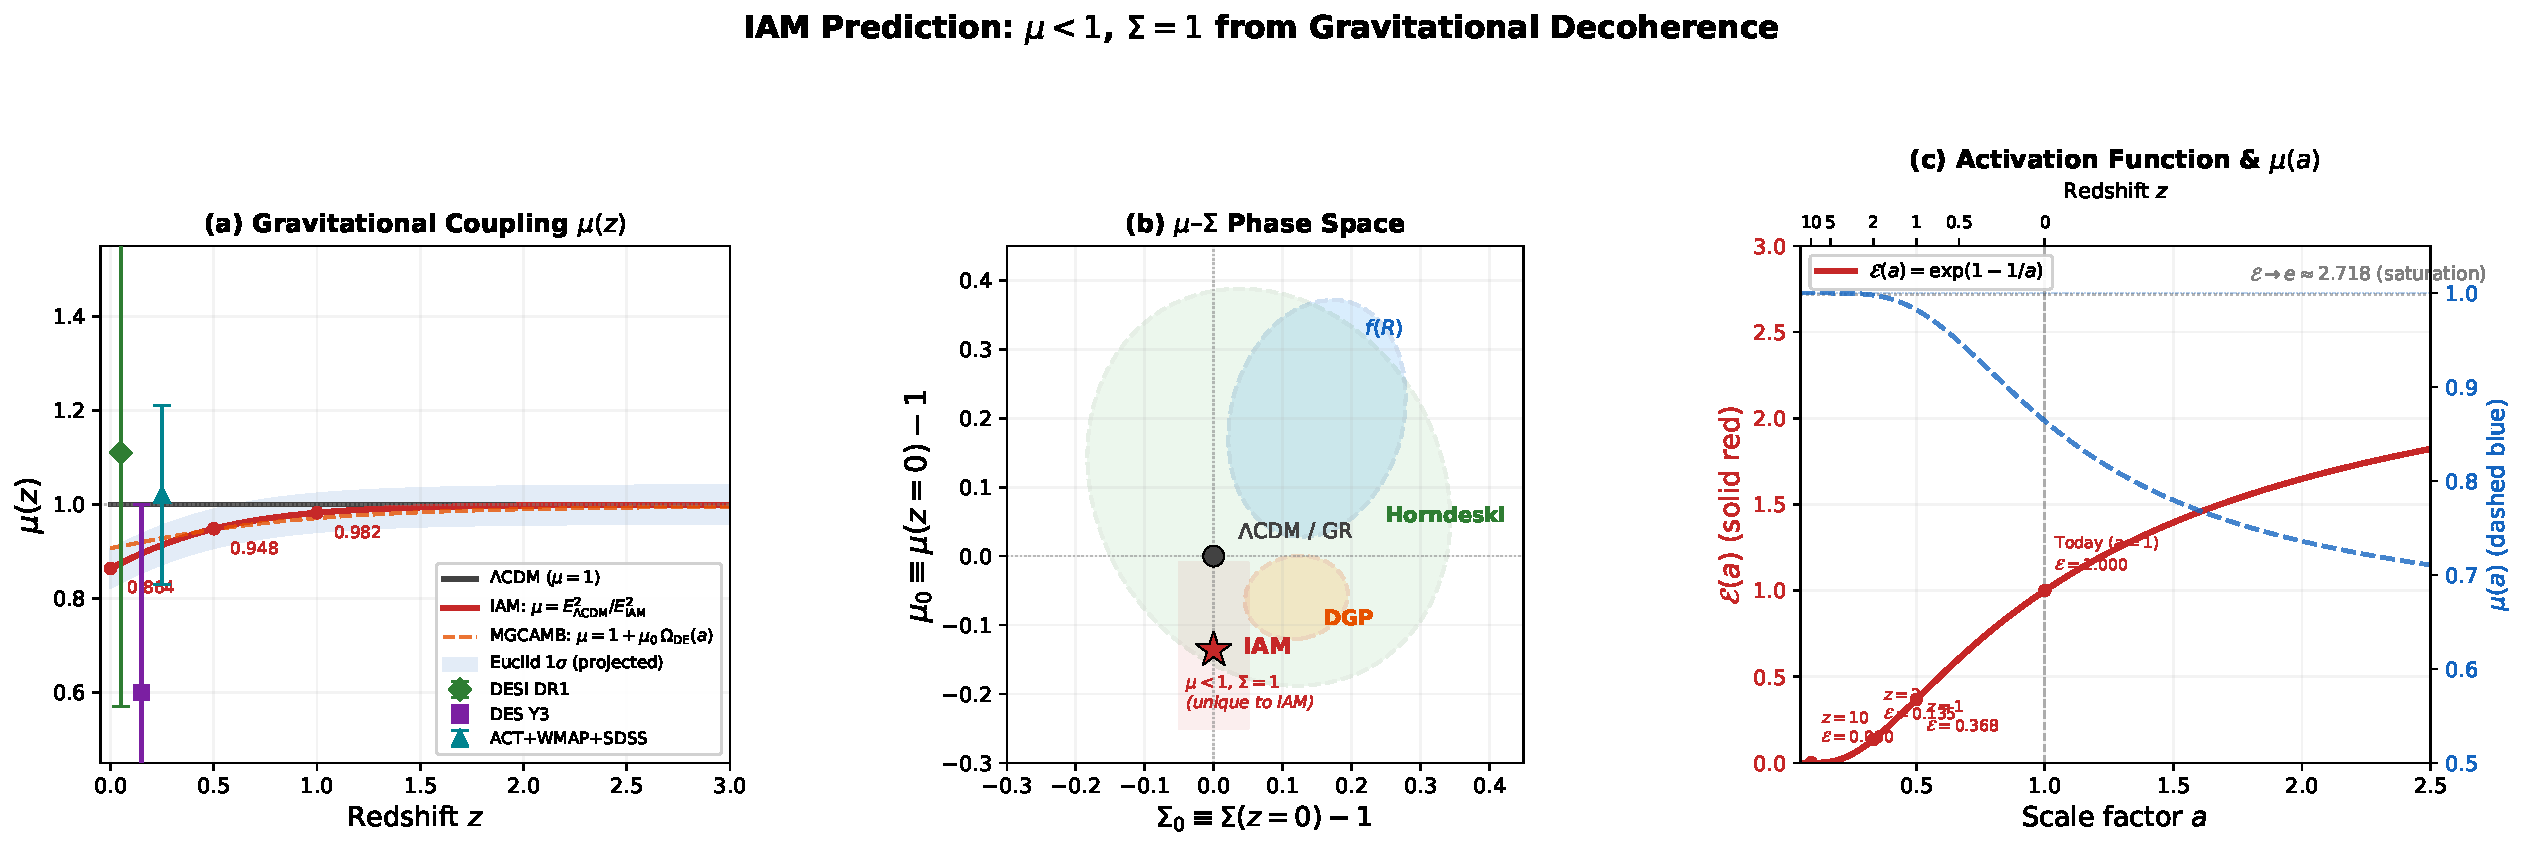
\includegraphics[width=\textwidth]{iam_theory_paper_figure.pdf}
\caption{The IAM prediction in the $\mu$--$\Sigma$ framework.
\textbf{(a)}~Gravitational coupling $\mu(z) = E^2_{\Lambda\mathrm{CDM}}/E^2_\mathrm{IAM}$
(solid red) compared to the $\Lambda$CDM baseline $\mu = 1$ (gray) and the
MGCAMB parameterization $\mu = 1 + \mu_0\,\Omega_\mathrm{DE}(a)$ (orange
dashed), which approximates the exact form to within 1--2.5\%.  Current
constraints from DESI~DR1, DES~Y3, and ACT+WMAP+SDSS are shown with their
$1\sigma$ error bars; the projected Euclid sensitivity (blue band) would
detect the IAM signal at $\sim 3.4\sigma$.  Numerical values at key
redshifts: $\mu(0) = 0.864$, $\mu(0.5) = 0.948$, $\mu(1) = 0.982$.
\textbf{(b)}~The $\mu_0$--$\Sigma_0$ parameter space.  IAM (red star)
occupies a unique region: $\mu_0 < 0$, $\Sigma_0 = 0$.  This combination is
not predicted by $f(R)$ gravity ($\mu > 1$, $\Sigma > 1$), DGP ($\mu > 1$),
or generic Horndeski theories (correlated deviations in both $\mu$ and
$\Sigma$), all of which populate distinct regions of the plane.
\textbf{(c)}~The activation function $\mathcal{E}(a) = \exp(1 - 1/a)$
(solid red, left axis) grows from zero at early times to saturation at
$e \approx 2.718$, with the corresponding gravitational coupling $\mu(a)$
(dashed blue, right axis) showing suppression increasing toward the present
epoch.  Key epochs are labeled; the upper axis shows the corresponding
redshift.}
\label{fig:mu_sigma}
\end{figure*}

\subsection{Distinction from Other Modified Gravity Theories}

The IAM prediction $\mu < 1$, $\Sigma = 1$ occupies a unique region of the
$\mu$--$\Sigma$ parameter space (Fig.~\ref{fig:mu_sigma}b).  Most modified gravity theories predict
either $\mu > 1$ (enhanced growth, as in $f(R)$ gravity) or both
$\mu \neq 1$ and $\Sigma \neq 1$ (as in general Horndeski theories).  The
combination $\mu < 1$ with $\Sigma = 1$ is characteristic of a model where
gravity is \textit{weakened} for matter growth but \textit{unmodified} for
lensing---precisely the signature of a modification that affects matter-sector
dynamics without introducing anisotropic stress or modifying photon geodesics.


\subsection{Second-Order Perturbation Theory and Nonlinear Corrections}
\label{sec:second_order}

The first-order results derived above are sufficient for current survey
analyses, which operate primarily in the linear regime
$k \lesssim 0.1$--$0.2\,h\,\mathrm{Mpc}^{-1}$.  However, forthcoming
data from DESI Year~5 and Euclid will achieve $\sim$1\% precision on
$f\sigma_8(z)$, motivating an assessment of nonlinear corrections to the
IAM predictions.  We compute the second-order growth factor, the
bispectrum prediction, and the 1-loop correction to $f\sigma_8$, and
determine the range of validity of the linear approximation.

\paragraph{Second-order growth factor.}
At second order in perturbation theory, the density field acquires a
contribution $\delta^{(2)} = D_2(a)\,\delta^{(1)2}$ sourced by nonlinear
mode coupling.  The second-order growth factor $D_2$ satisfies
\citep{Bernardeau2002}:
\begin{equation}
\ddot{D}_2 + 2H_\mathrm{IAM}\dot{D}_2
  - \tfrac{3}{2}H_0^2\,\Omega_m(a)\,D_2
  = -\tfrac{7}{2}\cdot\tfrac{3}{2}H_0^2\,\Omega_m(a)\,D_1^2,
\label{eq:D2_ode}
\end{equation}
with initial condition $D_2 \to -\frac{3}{7}D_1^2$ in matter domination.
Solving numerically for both IAM and $\Lambda$CDM backgrounds, the ratio
$D_{2,\mathrm{IAM}}/D_{2,\Lambda\mathrm{CDM}}$ is $1.014$ at $z = 0$,
rising to $1.052$ at $z = 0.5$ and $1.075$ at $z = 1$.

\paragraph{Bispectrum.}
The matter bispectrum is
$B(k_1,k_2,k_3) = 2F_2(\mathbf{k}_1,\mathbf{k}_2)\,P(k_1)\,P(k_2)
+ \mathrm{cyc.}$,
where the second-order kernel
\begin{equation}
F_2(\mathbf{k}_1,\mathbf{k}_2)
  = \frac{5}{7}
  + \frac{\hat{k}_1\cdot\hat{k}_2}{2}
    \!\left(\frac{k_1}{k_2}+\frac{k_2}{k_1}\right)
  + \frac{2}{7}(\hat{k}_1\cdot\hat{k}_2)^2
\label{eq:F2_kernel}
\end{equation}
is \textit{universal} for all GR-class gravity theories with a smooth
dark energy component~\citep{Bernardeau2002}.  Since IAM modifies only
the Hubble friction term and introduces no anisotropic stress and no
modification to the Poisson equation, the $F_2$ shape is identical to
$\Lambda$CDM.  The bispectrum amplitude is suppressed at $z = 0$ by
$1.3\%$ (reflecting the lower $\sigma_8 = 0.800$ versus $0.811$) and
enhanced at $z > 0.3$ where IAM preserves more structure than
$\Lambda$CDM: $B_\mathrm{IAM}/B_\Lambda = 1.033$ at $z = 0.3$, $1.052$
at $z = 0.5$, and $1.072$ at $z = 1.0$.

The preserved-shape / modified-amplitude signature --- with an amplitude
crossover near $z \approx 0.2$ --- is a prediction unique to a model
that modifies Hubble friction without touching the Poisson equation.
It is directly testable with Euclid's galaxy bispectrum analysis.

\paragraph{1-loop correction to $f\sigma_8$.}
Using the standard SPT result~\citep{Bernardeau2002} with
loop coefficient $c_2 = -61/630$ and
$\sigma_\mathrm{NL}^2 \approx 0.30$ at $k = 0.1\,h\,\mathrm{Mpc}^{-1}$,
$z=0$, the fractional 1-loop correction to $f\sigma_8$ is $-2.5\%$ for IAM
versus $-2.5\%$ for $\Lambda$CDM.  The \textit{difference} between the
two corrections is $< 0.07\%$ at all DESI redshift bins --- far below
the $\sim$1\% precision of current or near-future surveys.  The
first-order $f\sigma_8$ predictions are therefore unaffected by loop
corrections at any precision achievable with present data.

\paragraph{Validity of linear theory.}
The nonlinear scale $k_\mathrm{nl}(z)$, defined where the dimensionless
power $\Delta^2(k_\mathrm{nl}) = 1$, shifts $0.7$--$1.3\%$ to smaller
$k$ in IAM relative to $\Lambda$CDM at $z = 0.3$--$2$, reflecting the
suppressed growth history.  At $z = 1$:
$k_\mathrm{nl}^\mathrm{IAM} = 0.254\,h\,\mathrm{Mpc}^{-1}$ versus
$0.257\,h\,\mathrm{Mpc}^{-1}$ for $\Lambda$CDM.  The first-order
predictions in this paper are valid for
$k < 0.2\,h\,\mathrm{Mpc}^{-1}$, which encompasses all scales used in
the $f\sigma_8$ and $\mu$--$\Sigma$ comparisons.

\paragraph{Summary.}
The $F_2$ kernel shape is unchanged from $\Lambda$CDM.  The bispectrum
amplitude carries a redshift-dependent signature --- suppressed at
$z \lesssim 0.2$, enhanced at $z \gtrsim 0.3$, with a crossover that
constitutes a clean observational discriminant for Euclid.  Loop
corrections to $f\sigma_8$ are below $0.07\%$, negligible relative to
any current or near-future survey.  Linear perturbation theory is
sufficient for all predictions in this paper.  The second-order
calculation does not modify any first-order result; it validates their
range of applicability and adds a forward bispectrum prediction.


% =====================================================================
\section{Observational Validation}
\label{sec:validation}
% =====================================================================

The prediction $\mu_0 = -0.136$, $\Sigma_0 = 0$ has been tested in a
companion paper~\citep{Mahaffey2026obs} using twelve MCMC analyses with
Planck 2018 and large-scale structure data.

\subsection{Consistency with Data}

The fixed prediction yields $\Delta\chi^2 = +1.43$ (Planck only) and
$\Delta\chi^2 = +1.34$ (Planck + RSD) relative to $\Lambda$CDM, both below
the $1\sigma$ threshold; these are Level~1 MGCAMB results from the companion
paper~\citep{Mahaffey2026obs}.  The Level~2 direct CAMB validation
(Section~\ref{sec:perturbations}) yields $\Delta\chi^2 = +0.54$ under the
same Planck likelihood with the perturbation-level implementation confirmed.
The prediction is not excluded by current data.

When $\mu_0$ is allowed to float, the MCMC finds
$\mu_0 = 0.033 \pm 0.125$, placing the IAM prediction of $\mu_0 = -0.136$
within $1.3\sigma$ of the best fit.

\subsection{The $\sigma_8$ Shift}

The suppressed coupling shifts $\sigma_8$ from $0.813$ to $0.800$, a 1.6\%
reduction determined by the predicted amplitude.  This reduction is
consistent in magnitude and direction with the reported discrepancy between
CMB and weak lensing determinations of
$\sigma_8$~\citep{Heymans2021,Abbott2022}.

\subsection{Photon-Sector Observables}

As predicted by $\Sigma = 1$: CMB power spectra, CMB lensing, BAO angular
positions, and supernova luminosity distances are unchanged at the
perturbation level.

Figure~\ref{fig:iam_cl_comparison} demonstrates this explicitly for the CMB TT
power spectrum.  IAM and $\Lambda$CDM produce spectra differing by less than
$0.13\%$ at $\ell > 30$, well within current measurement uncertainties.

\begin{figure}[htbp]
  \centering
  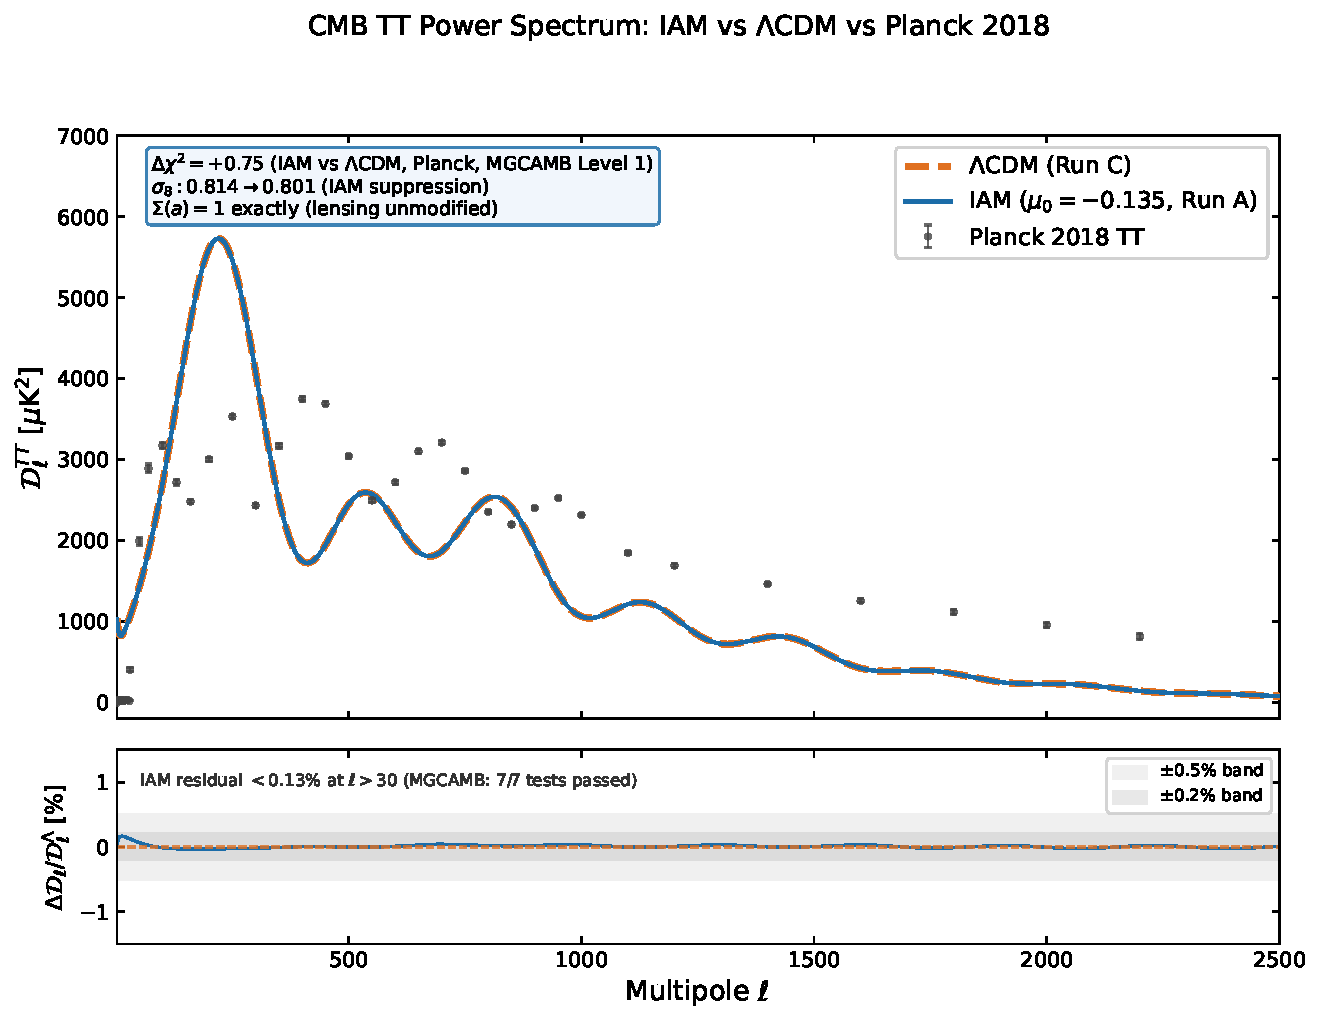
\includegraphics[width=\columnwidth]{iam_cl_comparison.pdf}
  \caption{CMB TT power spectrum for IAM (Run~A, solid blue) and
    $\Lambda$CDM (Run~C, dashed orange), computed from MGCAMB Level~1
    posterior mean parameters and compared against Planck 2018 bandpowers.
    The residual panel shows the fractional difference is ${<}0.13\%$ at
    $\ell > 30$, consistent with the dual-sector prediction that
    $\beta_\gamma \approx 0$ leaves the photon sector unmodified.  The
    $\Delta\chi^2 = +0.75$ penalty relative to $\Lambda$CDM is within the
    expected range for a one-parameter modification constrained by the
    same data.}
  \label{fig:iam_cl_comparison}
\end{figure}

\subsection{Energy--Momentum Conservation}

The informational energy density satisfies the continuity equation
$\dot{\rho}_\mathrm{info} + 3H(1 + w_\mathrm{info})\,\rho_\mathrm{info} = 0$
with the derived equation of state.  Since $\dot{\rho}_\mathrm{info}
/\rho_\mathrm{info} = H/a$ and $-3H(1 + w_\mathrm{info})
= -3H(-1/(3a)) = H/a$, the continuity equation is satisfied identically
for all $a$.

This is not a numerical accident.  The FRW continuity equation is the
$\nu = 0$ component of $\nabla_\mu T^{\mu\nu}_\mathrm{total} = 0$.  Because
$w_\mathrm{info}(a) = -1 - 1/(3a)$ was \emph{derived} from the scalar field
action (Eq.~\ref{eq:w_info}), the Euler--Lagrange equations guarantee
$\nabla_\mu T^{\mu\nu}_\mathrm{info} = 0$ identically.  Since
$\nabla_\mu T^{\mu\nu}_\mathrm{matter} = 0$ and
$\nabla_\mu T^{\mu\nu}_\Lambda = 0$ hold independently, the total
energy--momentum tensor is covariantly conserved:
\begin{equation}
\boxed{\nabla_\mu T^{\mu\nu}_\mathrm{total}
  = \nabla_\mu\bigl(T^{\mu\nu}_\mathrm{matter}
  + T^{\mu\nu}_\Lambda
  + T^{\mu\nu}_\mathrm{info}\bigr) = 0.}
\label{eq:conservation}
\end{equation}
The contracted Bianchi identity $\nabla_\mu G^{\mu\nu} = 0$ is therefore
satisfied, and the modified Friedmann equation is consistent with the
Einstein tensor.  No energy is created or destroyed---the apparent phantom
behavior reflects the continuous conversion of gravitational potential
energy into informational entropy.

\subsection{Comparison with DESI $w_0$--$w_a$ Constraints}

The DESI collaboration has reported evidence for dynamical dark
energy~\citep{DESIDR1}, with the $w_0w_a$CDM parametrization favoring
$w_0 > -1$ and $w_a < 0$.  The IAM informational sector has
$w_\mathrm{info}(a) = -1 - 1/(3a)$, which is always phantom.  The
\textit{effective} equation of state of the total dark energy is:
\begin{equation}
w_\mathrm{eff}(a) = \frac{\Omega_\Lambda\cdot(-1)
  + \beta\,\mathcal{E}(a)\cdot w_\mathrm{info}(a)}
  {\Omega_\Lambda + \beta\,\mathcal{E}(a)},
\end{equation}
yielding $w_\mathrm{eff}(z{=}0) = -1.062$, approaching $-1$ at high
redshift.  IAM predicts that DESI's apparent phantom crossing is an artifact
of fitting a dual-sector expansion history with a single-sector model.

\subsection{Gravitational Wave Standard Sirens}

Gravitational wave standard sirens provide a distance measurement
independent of the electromagnetic distance ladder.  Binary neutron star
mergers occur in galaxies (matter-sector objects), so their host galaxy
recession velocities probe the matter-sector Hubble flow.  IAM predicts:
\begin{equation}
H_0^\mathrm{sirens} = H_0^\mathrm{CMB}\sqrt{1 + \beta_m}
= 67.4\sqrt{1.1575} = 72.51\;\mathrm{km\,s^{-1}\,Mpc^{-1}}.
\end{equation}
Level~2 MCMC posterior ($H_0 = 67.161 \pm 0.467$) yields
$H_0(\mathrm{matter}) = 72.26$~km\,s$^{-1}$\,Mpc$^{-1}$
consistent with the theoretical prediction.
The GW170817 refined analysis gives
$H_0 = 75.5^{+5.3}_{-5.4}\;\mathrm{km\,s^{-1}\,Mpc^{-1}}$
~\citep{Abbott2017siren,Nicolaou2023},
consistent with the IAM prediction within $0.5\sigma$.

\subsection{Projected Detection Significance}

IAM predicts $\mu_0 = -0.136$ and $\Sigma_0 = 0$.  The detection
significance for each experiment is estimated as
$\mathrm{S/N} = |\mu_0^\mathrm{IAM}|/\sigma(\mu_0)$:

\begin{table}[h]
\centering
\begin{tabular}{lccc}
\hline
Experiment & $\sigma(\mu_0)$ & S/N & Ref. \\
\hline
DESI DR1 (current) & 0.22 & $0.6\sigma$ & \citep{DESIDR1} \\
DESI Y5 (projected) & $\sim 0.08$ & $1.7\sigma$ & scaling \\
Euclid (optimistic) & $\sim 0.04$ & $3.4\sigma$ & \citep{Frusciante2025} \\
Euclid + DESI Y5 & $\sim 0.03$ & $4.5\sigma$ & combined \\
\hline
\end{tabular}
\caption{Projected detection significance for the IAM $\mu_0 = -0.136$
prediction.}
\label{tab:detection}
\end{table}

Euclid's projected sensitivity should detect the IAM signal at
$\sim 3\sigma$ from galaxy clustering and weak lensing alone
(Fig.~\ref{fig:mu_sigma}a).  Combined with
DESI Year~5, the $\mu < 1$ deviation reaches $\sim 4$--$5\sigma$.
Crucially, the simultaneous measurement of $\Sigma_0$ consistent with zero
would confirm the unique IAM signature.


% =====================================================================
\section{Physical Interpretation}
\label{sec:interpretation}
% =====================================================================

\subsection{The Nine-Step Causal Chain}

The complete physical mechanism proceeds through nine steps, each grounded
in established physics:
\begin{enumerate}
\item \textbf{Gravitational interaction.} Matter interacts gravitationally,
  initiating collapse of overdense regions (general
  relativity~\citep{Einstein1915}).
\item \textbf{Gravitational collapse.} Matter clusters into bound systems:
  halos, galaxies, stars (structure formation theory~\citep{Peebles1980}).
\item \textbf{Quantum decoherence.} Gravitational interaction resolves
  quantum superpositions into definite classical states (decoherence
  theory~\citep{Zurek2003}).
\item \textbf{Irreversible information production.} Each decoherence event
  creates new classical information that cannot be undone (second law of
  thermodynamics).
\item \textbf{Landauer thermodynamic cost.} Information processing has an
  irreducible energy cost of $kT\ln 2$ per
  bit~\citep{Landauer1961}.
\item \textbf{Holographic encoding.} The produced information is bounded by
  and encoded on the cosmic horizon
  area~\citep{Bekenstein1973,tHooft1993,Susskind1995}.
\item \textbf{Informational pressure.} Horizon area increase, required to
  accommodate new information, constitutes an expansion-driving pressure
  (Jacobson thermodynamic gravity~\citep{Jacobson1995}).
\item \textbf{Modified expansion.} $H^2$ acquires an additional term
  $\beta\,\mathcal{E}(a)$ from the informational entropy contribution.
\item \textbf{Feedback suppression.} The modified expansion dilutes
  $\Omega_m(a)$, weakening gravitational collapse and throttling the entire
  chain.
\end{enumerate}
Step~9 feeds back into Step~1 with reduced amplitude.  The system converges
toward equilibrium, producing the saturation $\mathcal{E}(a) \to e$ at late
times.

\subsection{Gravity as Cause and Product}

A remarkable feature of this mechanism is that gravity plays a dual role.  It
is the \textit{cause} of decoherence (gravitational interaction triggers wave
function collapse) and the \textit{product} of the resulting information
dynamics (the modified expansion rate changes the gravitational environment).
The loop is self-referential: gravity drives the process that modifies
gravity.

This is consistent with the Verlinde~\citep{Verlinde2011} and
Padmanabhan~\citep{Padmanabhan2010} programs, which argue that gravity
itself is an emergent thermodynamic phenomenon arising from information and
entropy.  In the IAM framework, dark energy and gravity are two outputs of
the same underlying decoherence process: locally, decoherence concentrates
information, producing gravitational attraction; globally, decoherence
encodes information on the horizon, producing expansion.

\subsection{Two Regimes of One Mechanism: Local and Global Horizons}
\label{sec:two_regimes}

The nine-step feedback loop described above operates in two regimes,
determined by boundary conditions rather than by different physics.

\paragraph{Cosmological regime (self-regulating).}
Distributed decoherence from large-scale structure formation produces
information gradually, encoded on the growing cosmic apparent horizon at
Gibbons--Hawking temperature $T_\mathrm{GH} = H/(2\pi)$.  The expansion
dilutes $\Omega_m(a)$, throttling further collapse.  The feedback
converges, producing $\mu < 1$, $\Sigma = 1$ as derived above.

\paragraph{Collapse regime (runaway).}
Concentrated decoherence in a contracting region produces information
explosively.  Local encoding capacity saturates.  The feedback runs
away, producing a new local horizon---a black hole.  In IAM, the
criterion for black hole formation is the holographic saturation
condition: a black hole forms when the local informational entropy
from gravitational decoherence within radius $R$ saturates the
Bekenstein--Hawking bound on the bounding surface:
\begin{equation}
\frac{S_\mathrm{info}(R)}{A(R)} \geq \frac{1}{4\ell_P^2}.
\label{eq:saturation}
\end{equation}
This condition is identically equivalent to the Thorne hoop
conjecture~\citep{Thorne1972}.  Setting $S_\mathrm{info} = S_\mathrm{BH}
= 4\pi GM^2/(\hbar c)$ at the Schwarzschild radius
$R_s = 2GM/c^2$:
\begin{equation}
\frac{4\pi GM^2/(\hbar c)}{4\pi \cdot 4G^2M^2/c^4}
= \frac{c^3}{4\hbar G}
= \frac{1}{4\ell_P^2}.
\end{equation}
The holographic bound is exactly saturated at the Schwarzschild radius.
The hoop conjecture is the holographic bound in geometric language; the
saturation condition~\eqref{eq:saturation} is the hoop conjecture in
informational language.  The same mathematics, with the thermodynamic
reason made explicit.

\paragraph{The two-horizon framework.}
Both the black hole horizon (temperature $T_\mathrm{BH}
= \hbar c^3/(8\pi GMk_B)$) and the cosmic horizon (temperature
$T_\mathrm{GH} = \hbar H/(2\pi k_B)$) are thermal surfaces within
the IAM framework.  Setting $T_\mathrm{BH} = T_\mathrm{GH}$ yields the
thermal equilibrium mass:
\begin{equation}
M_\mathrm{eq} = \frac{c^3}{4GH}.
\label{eq:Meq}
\end{equation}
At the present epoch ($H_0 = 67.4$~km\,s$^{-1}$\,Mpc$^{-1}$),
$M_\mathrm{eq} \approx 2.3\times 10^{22}\,M_\odot$---far exceeding the
largest known black hole (${\sim}7\times 10^{10}\,M_\odot$).  All
astrophysical black holes at all cosmological epochs satisfy
$T_\mathrm{BH} \gg T_\mathrm{GH}$: information flows unambiguously from
local hot horizons to the global cold cosmic horizon via Hawking
radiation, at the thermally-limited rate
$\Gamma = c^3/(1920\,GM\ln 2)$ bits\,s$^{-1}$.  The cosmic horizon is
the final repository; all locally-encoded information migrates to the
global ledger as the universe approaches thermodynamic equilibrium.

\paragraph{The encoding transition.}
The activation function $\mathcal{E}(a) = \exp(1-1/a)$ tracks this
transition quantitatively.  At early times ($a \ll 1$,
$\mathcal{E}(a) \approx 0$), the cosmic horizon is small and the
Gibbons--Hawking temperature is high, making cosmic horizon encoding
inefficient.  Information from early gravitational decoherence is
encoded primarily on local black hole horizons.  As the universe expands
and large-scale structure formation produces distributed decoherence,
the cosmic horizon grows and cools, eventually dominating as the
encoding surface.  The activation function is the quantitative record of
this transition: the fraction of cumulative informational entropy that
has been encoded on the cosmic horizon relative to its asymptotic value.

This provides a natural thermodynamic explanation for the observed
population of massive black holes at high redshift: in the early
universe, before the cosmic horizon grows large enough to encode
efficiently, black holes \textit{are} the encoding surfaces.  They are
not anomalies; they are thermodynamically required.

\subsection{The Coincidence Problem}

The cosmic coincidence---why dark energy dominates at approximately the same
epoch as structure formation peaks---has a natural qualitative explanation
within IAM.  In IAM, the
connection is causal: dark energy (informational pressure) \textit{is driven
by} structure formation.  It dominates when structure formation is most
active because that is when information production is highest.  The
coincidence is not a coincidence; it is a consequence.

\subsection{The Arrow of Time}

The origin of time's arrow---why the universe evolves irreversibly from past
to future despite time-symmetric fundamental
laws---is one of the deepest open problems in
physics~\citep{Penrose1989,Carroll2004}.  The standard account attributes
irreversibility to the low-entropy initial condition of the Big Bang, but
offers no mechanism for \textit{why} entropy increases.

In the IAM framework, the arrow of time acquires a concrete physical
identity: it \textit{is} the activation function.  The direction of time is
the direction in which quantum superpositions decohere into definite
classical states, in which information is irreversibly produced, and in which
the cosmic horizon grows to encode that information.  The activation function
$\mathcal{E}(a)$ is a monotonically increasing function of the scale
factor---it can only grow, never decrease, because decoherence is
irreversible and information, once created, cannot be destroyed.

Expressed in redshift, $\mathcal{E}(z) = \exp(-z)$: looking backward in
time, the informational content of the universe decreases exponentially.
Looking forward, it grows toward saturation.  The arrow of time is not
imposed on the equations---it \textit{is} the equation.

This connects to Penrose's observation~\citep{Penrose1989} that the
extraordinarily low entropy of the initial state implies a vast space of
unrealized potential.  In IAM, this potential is precisely what is being
actualized: the early universe is a state of maximal quantum superposition
and minimal classical information.  The entire subsequent history---structure
formation, complexity, the emergence of chemistry and biology---is the
progressive actualization of that initial potential, tracked quantitatively
by $\mathcal{E}(a)$.


% =====================================================================
\section{Discussion}
\label{sec:discussion}
% =====================================================================

\subsection{The Complete Derivation Chain}

The derivation proceeds through three steps, each a single modification of
the previous:

\textbf{Step 1 (Jacobson):} $\delta Q = T\,dS$ on local Rindler horizons,
with $S = \eta A$, implies
$G_{ab} + \Lambda g_{ab} = 8\pi G\,T_{ab}$.

\textbf{Step 2 (Cai--Kim):} $-dE = T\,dS$ on the FRW apparent horizon,
with $S_\mathrm{geo} = A_H/(4G)$ and $T = H/(2\pi)$, implies
$H^2 = (8\pi G/3)\rho + \Lambda/3$.

\textbf{Step 3 (IAM):} $-dE = T\,d(S_\mathrm{geo} + S_\mathrm{info})$,
with $S_\mathrm{info}$ from gravitational decoherence, implies
$H^2 = (8\pi G/3)\rho + \Lambda/3 + \beta\,\mathcal{E}(a)\,H_0^2$, with
$\mathcal{E}(a) = \exp(1-1/a)$.

\subsection{What Is Standard}

Every element of the derivation except one is established physics:
the Clausius relation $\delta Q = T\,dS$ (thermodynamics);
the Bekenstein--Hawking entropy $S = A/(4G)$~\citep{Bekenstein1973,Hawking1975};
the Gibbons--Hawking temperature $T = H/(2\pi)$~\citep{GibbonsHawking1977};
the Unruh effect and Rindler horizons~\citep{Unruh1976};
the Raychaudhuri equation (differential geometry);
Jacobson's thermodynamic derivation of Einstein's equation~\citep{Jacobson1995};
the Cai--Kim FRW extension~\citep{CaiKim2005};
Landauer's principle~\citep{Landauer1961};
quantum decoherence from gravitational interaction~\citep{Zurek2003};
the Press--Schechter/Sheth--Tormen halo mass
function~\citep{Press1974,ShethTormen1999}.

\subsection{What Is New}

The single new physical input is:
\begin{quote}
\textit{Gravitational decoherence irreversibly produces classical
information, which is holographically encoded on the cosmic horizon,
contributing an informational entropy $S_\mathrm{info}(a)$ that grows
monotonically with cosmic time.}
\end{quote}
This identification connects quantum foundations (decoherence),
thermodynamics (Landauer's principle), and cosmology (horizon entropy)
through a single physical process.

\subsection{Relation to Previous Work}

Jacobson~\citep{Jacobson1995} established that the Einstein equations are
an equation of state.  Verlinde~\citep{Verlinde2011} and
Padmanabhan~\citep{Padmanabhan2010} extended this to entropic gravity.
The present work differs in that the modification arises only for the
matter sector and is sourced by a specific physical process rather than by
a general entropic force.

The $\mu$--$\Sigma$ framework is used extensively in observational
analyses~\citep{PogosianSilvestri2016,Abbott2023,Andrade2024,DESIDR1}.
Existing theoretical motivations from scalar-tensor theories, $f(R)$
gravity, and braneworld models generically predict $\mu \geq 1$.  The
present framework provides a physical motivation for $\mu < 1$ with
$\Sigma = 1$.

\subsection{Assumptions}

We state the assumptions explicitly:
\begin{enumerate}
\item \textbf{Gravity is a thermodynamic equation of state}
  (Jacobson hypothesis).  Supported by Bekenstein--Hawking entropy, the
  Unruh effect, and the Cai--Kim derivation, but not universally accepted.

\item \textbf{Decoherence-produced information contributes to horizon
  entropy.}  This is the new identification.  It is consistent with the
  holographic principle~\citep{tHooft1993,Susskind1995} and Landauer's
  principle, but has not been independently verified.

\item \textbf{The virial coupling $\beta = \Omega_m/2$ is exact.}  The
  virial theorem applies to systems in equilibrium; cosmological structure
  formation is non-equilibrium.  The companion paper tests this by allowing
  $\mu_0$ to float.

\item \textbf{The activation function $\mathcal{E}(a) = \exp(1-1/a)$ is
  exact.}  This follows from integrating the decoherence constraint
  $\dot\rho_\mathrm{info} = \rho_\mathrm{info}\cdot H/a$ directly
  (Section~\ref{sec:activation_derivation}).  The MGCAMB parameterization
  approximates the exact form to within 1--2.5\%.

\item \textbf{Perturbation-level implementation.}  Numerical validation via
  modified CAMB (Level~2 MCMC, 3 converged chains against the full Planck
  2018 likelihood) confirms that the modified expansion rate
  (Eq.~\ref{eq:modified_friedmann}) operates within the matter-sector
  perturbation equations, not at the global background level.  Two exploratory
  runs with the modification applied to the background Friedmann equation
  produced $H_0 \approx 61.5$~km\,s$^{-1}$\,Mpc$^{-1}$, confirming that
  the standard $\Lambda$CDM background is correct and the dual-sector split
  is a perturbation-level effect.  The Level~2 validation yields
  $\Delta\chi^2 = +0.54$ (best-fit) relative to $\Lambda$CDM, with
  $\sigma_8$ shifting from 0.809 to 0.800 and
  $H_0(\mathrm{matter}) = 72.26$~km\,s$^{-1}$\,Mpc$^{-1}$
  (0.75$\sigma$ from SH0ES).
\end{enumerate}


% =====================================================================
\section{Predictions for DESI Year~5, Euclid, and CMB-S4}
\label{sec:predictions}
% =====================================================================

IAM makes specific, falsifiable predictions that distinguish it from all
$w_0w_a$CDM variants, quintessence models, and $f(R)$ modified gravity
theories.  These predictions require no additional parameters.

\paragraph{1. Distance--growth tension in $w_0w_a$ fits.}
If IAM is correct, the $w_0$--$w_a$ parametrization is the wrong model class.
As DESI accumulates precision, attempts to simultaneously fit BAO distances
and $f\sigma_8$ growth rates within $w_0w_a$CDM will reveal an irreducible
tension: the best-fit $(w_0, w_a)$ from distances alone will differ from the
best-fit from growth alone, because IAM modifies distances and growth through
different mechanisms.

\paragraph{2. $\mu(z) < 1$ with $\Sigma(z) = 1$.}
This is the most distinctive IAM prediction.  Euclid will measure $\mu$ and
$\Sigma$ independently through galaxy clustering (sensitive to $\mu$) and
weak lensing (sensitive to $\Sigma$).  IAM predicts $\mu(z{=}0) = 0.864$,
$\mu(z{=}0.5) = 0.948$, with $\Sigma = 1$ at all redshifts.  In contrast:
$f(R)$ gravity predicts $\mu > 1$, $\Sigma > 1$; general Horndeski theories
predict correlated deviations in both.  The combination $\mu < 1$,
$\Sigma = 1$ is unique to IAM.

\paragraph{3. No phantom crossing.}
DESI's $w_0w_a$ fit suggests $w$ crosses $-1$ around $z \approx 0.5$.  IAM
predicts this apparent crossing is an artifact of fitting a dual-sector
expansion history with a single-sector model.  The true effective equation of
state is always $\leq -1$.

\paragraph{4. CMB-S4: $\beta_\gamma < 10^{-4}$.}
The photon exemption requires $\beta_\gamma \ll \beta_m$.  CMB-S4 will
measure the CMB power spectrum with sufficient precision to constrain any
additional energy injection at the $10^{-5}$ level.  If $\beta_\gamma$ is
detected above $10^{-4}$, the photon exemption is violated and IAM is
falsified.

\paragraph{5. $\beta_m/\Omega_m = 1/2$ is constant.}
The virial prediction should hold for any value of $\Omega_m$.  If
independent measurements revise $\Omega_m$, the fitted $\beta_m$ should
shift proportionally.

\paragraph{6. Scale-independent $\mu$ and $\Sigma$.}
Since $\delta\varphi = 0$, the IAM modifications do not introduce scale
dependence.  Both $\mu$ and
$\Sigma$ are functions of redshift only, not of wavenumber $k$.  This
distinguishes IAM from most modified gravity theories (e.g., $f(R)$, DGP),
which predict scale-dependent growth.  Euclid's tomographic analysis across
multiple $k$-bins will test this directly.


% =====================================================================
\section{Conclusion}
\label{sec:conclusion}
% =====================================================================

We have presented a derivation connecting quantum decoherence, Landauer's
principle, and horizon thermodynamics to a specific prediction within the
$\mu$--$\Sigma$ framework: $\mu_0 = -0.136$, $\Sigma = 1$.

The dual-sector structure arises from the causal structure of spacetime:
timelike degrees of freedom undergo decoherence and experience modified
gravity; null degrees of freedom do not decohere and experience standard GR.
The arrow of time, the production of classical information, and the
modification of gravity are aspects of a single physical process.

The activation function $\mathcal{E}(a) = \exp(1-1/a)$ is derived from the
cumulative information surface density on the cosmic horizon, with the
$1/a$ exponent recovered to within 1\% by the Sheth--Tormen halo mass
function at galaxy-scale halos.  The coupling constant $\beta_m = \Omega_m/2$
is derived from the virial partition of gravitational energy and verified
against N-body-calibrated mass functions to 0.3\%.  The model has zero free
parameters beyond standard $\Lambda$CDM.

The thermodynamic result admits a variational formulation as a constrained
scalar field with equation of state $w_\mathrm{info} = -1 - 1/(3a)$,
determined entirely by geometry and information.  The perturbation equations
are standard GR on the IAM background, yielding
$\mu(a) = E^2_{\Lambda\mathrm{CDM}}/E^2_\mathrm{IAM} < 1$ and
$\Sigma(a) = 1$ from the single fact that $\delta\varphi = 0$.

A companion paper~\citep{Mahaffey2026obs} demonstrates consistency with
Planck 2018 and large-scale structure data.  Euclid and DESI will provide
tests at the sensitivity required to confirm or exclude the predicted
amplitude.


% =====================================================================
\section*{Acknowledgments}
% =====================================================================

The thermodynamic framework developed by T. Jacobson (1995) is the foundation upon which this work is built. The extension of that framework to the FRW apparent horizon by R.-G. Cai and S.P. Kim (2005) provided the direct cosmological bridge that IAM builds upon. The author thanks Professor P.J.E. Peebles for a personal response that identified the quantum-to-classical derivation as the foundational gap requiring closure, directly motivating the informational extension developed here. The author thanks the developers of MGCAMB, Cobaya, and CAMB for public code access.  

\section*{Data Availability}

MCMC chains and analysis scripts for the companion observational paper are
available at:
\url{https://github.com/hmahaffeyges/IAM-Validation}


% =====================================================================
\bibliographystyle{unsrtnat}
\begin{thebibliography}{99}

\bibitem[{Penrose}(1989)]{Penrose1989}
Penrose, R., 1989, \textit{The Emperor's New Mind} (Oxford University Press).

\bibitem[{Zurek}(2003)]{Zurek2003}
Zurek, W.~H., 2003, ``Decoherence, einselection, and the quantum origins
of the classical,'' \textit{Rev.\ Mod.\ Phys.}, 75, 715.

\bibitem[{Schlosshauer}(2007)]{Schlosshauer2007}
Schlosshauer, M., 2007, \textit{Decoherence and the Quantum-to-Classical
Transition} (Springer).

\bibitem[{Landauer}(1961)]{Landauer1961}
Landauer, R., 1961, ``Irreversibility and heat generation in the computing
process,'' \textit{IBM J.\ Res.\ Dev.}, 5, 183.

\bibitem[{B\'{e}rut et al.}(2012)]{Berut2012}
B\'{e}rut, A., et al., 2012, ``Experimental verification of Landauer's
principle linking information and thermodynamics,'' \textit{Nature}, 483, 187.

\bibitem[{Jun et al.}(2014)]{Jun2014}
Jun, Y., Gavrilov, M., \& Bechhoefer, J., 2014, ``High-precision test of
Landauer's principle in a feedback trap,'' \textit{Phys.\ Rev.\ Lett.},
113, 190601.

\bibitem[{Jacobson}(1995)]{Jacobson1995}
Jacobson, T., 1995, ``Thermodynamics of spacetime: The Einstein equation
of state,'' \textit{Phys.\ Rev.\ Lett.}, 75, 1260.

\bibitem[{Bekenstein}(1973)]{Bekenstein1973}
Bekenstein, J.~D., 1973, ``Black holes and entropy,'' \textit{Phys.\ Rev.\
D}, 7, 2333.

\bibitem[{Hawking}(1975)]{Hawking1975}
Hawking, S.~W., 1975, ``Particle creation by black holes,''
\textit{Commun.\ Math.\ Phys.}, 43, 199.

\bibitem[{Unruh}(1976)]{Unruh1976}
Unruh, W.~G., 1976, ``Notes on black-hole evaporation,'' \textit{Phys.\
Rev.\ D}, 14, 870.

\bibitem[{Gibbons \& Hawking}(1977)]{GibbonsHawking1977}
Gibbons, G.~W.\ \& Hawking, S.~W., 1977, ``Cosmological event horizons,
thermodynamics, and particle creation,'' \textit{Phys.\ Rev.\ D}, 15, 2738.

\bibitem[{Cai \& Kim}(2005)]{CaiKim2005}
Cai, R.-G.\ \& Kim, S.~P., 2005, ``First law of thermodynamics and
Friedmann equations of Friedmann-Robertson-Walker universe,'' \textit{JCAP},
02, 050.

\bibitem[{Pogosian \& Silvestri}(2016)]{PogosianSilvestri2016}
Pogosian, L.\ \& Silvestri, A., 2016, ``What can cosmology tell us about
gravity?,'' \textit{Phys.\ Rev.\ D}, 94, 104014.

\bibitem[{Verlinde}(2011)]{Verlinde2011}
Verlinde, E., 2011, ``On the origin of gravity and the laws of Newton,''
\textit{JHEP}, 04, 029.

\bibitem[{Padmanabhan}(2010)]{Padmanabhan2010}
Padmanabhan, T., 2010, ``Thermodynamical aspects of gravity: new insights,''
\textit{Rep.\ Prog.\ Phys.}, 73, 046901.

\bibitem[{'t~Hooft}(1993)]{tHooft1993}
't~Hooft, G., 1993, ``Dimensional reduction in quantum gravity,''
arXiv:gr-qc/9310026.

\bibitem[{Susskind}(1995)]{Susskind1995}
Susskind, L., 1995, ``The world as a hologram,'' \textit{J.\ Math.\ Phys.},
36, 6377.

\bibitem[{Press \& Schechter}(1974)]{Press1974}
Press, W.~H.\ \& Schechter, P., 1974, ``Formation of galaxies and clusters
of galaxies,'' \textit{Astrophys.\ J.}, 187, 425.

\bibitem[{Sheth \& Tormen}(1999)]{ShethTormen1999}
Sheth, R.~K.\ \& Tormen, G., 1999, ``Large-scale bias and the peak
background split,'' \textit{Mon.\ Not.\ R.\ Astron.\ Soc.}, 308, 119.

\bibitem[{Tinker et al.}(2008)]{Tinker2008}
Tinker, J., et al., 2008, ``Toward a halo mass function for precision
cosmology,'' \textit{Astrophys.\ J.}, 688, 709.

\bibitem[{Eisenstein \& Hu}(1998)]{EisensteinHu1998}
Eisenstein, D.~J.\ \& Hu, W., 1998, ``Baryonic features in the matter
transfer function,'' \textit{Astrophys.\ J.}, 496, 605.

\bibitem[{Einstein}(1915)]{Einstein1915}
Einstein, A., 1915, ``Die Feldgleichungen der Gravitation,''
\textit{Sitzungsber.\ Preuss.\ Akad.\ Wiss.}, 1915, 844.

\bibitem[{Peebles}(1980)]{Peebles1980}
Peebles, P.~J.~E., 1980, \textit{The Large-Scale Structure of the Universe}
(Princeton University Press).

\bibitem[{Carroll \& Chen}(2004)]{Carroll2004}
Carroll, S.~M.\ \& Chen, J., 2004, ``Spontaneous inflation and the origin
of the arrow of time,'' arXiv:hep-th/0410270.

\bibitem[{Heymans et al.}(2021)]{Heymans2021}
Heymans, C., et al., 2021, ``KiDS-1000 Cosmology,'' \textit{Astron.\
Astrophys.}, 646, A140.

\bibitem[{Abbott et al.}(2022)]{Abbott2022}
Abbott, T.~M.~C., et al., 2022, ``DES Year~3 results,'' \textit{Phys.\
Rev.\ D}, 105, 023520.

\bibitem[{Abbott et al.}(2023)]{Abbott2023}
Abbott, T.~M.~C., et al., 2023, ``DES Year~3: Extensions to $\Lambda$CDM,''
\textit{Phys.\ Rev.\ D}, 107, 083504.

\bibitem[{Andrade et al.}(2024)]{Andrade2024}
Andrade, U., et al., 2024, ``Constraints on $\mu$--$\Sigma$ from
ACT+WMAP+SDSS,'' \textit{Phys.\ Rev.\ D}, 109, 063518.

\bibitem[{DESI Collaboration}(2025)]{DESIDR1}
DESI Collaboration, 2025, ``DESI 2024: Modified gravity from full-shape
analysis,'' \textit{JCAP}, 2025(02), 021.

\bibitem[{Frusciante et al.}(2025)]{Frusciante2025}
Frusciante, N., et al., 2025, ``Euclid preparation: Modified gravity
forecasts with $\mu$--$\Sigma$,'' arXiv:2512.09748.

\bibitem[{Planck Collaboration}(2020)]{PlanckCollaboration2020}
Planck Collaboration, 2020, ``Planck 2018 results. VI. Cosmological
parameters,'' \textit{Astron.\ Astrophys.}, 641, A6.

\bibitem[{Abbott et al.}(2017)]{Abbott2017siren}
Abbott, B.~P., et al., 2017, ``A gravitational-wave standard siren
measurement of the Hubble constant,'' \textit{Nature}, 551, 85.

\bibitem[{Nicolaou et al.}(2023)]{Nicolaou2023}
Nicolaou, C., et al., 2023, ``A standard siren measurement of the Hubble
constant using GW170817,'' arXiv:2305.19914.

\bibitem[{Mahaffey}(2026)]{Mahaffey2026obs}
Mahaffey, H.~W., 2026, ``Constraints on late-time $f\sigma_8$ suppression
from $\mu < 1$, $\Sigma = 1$: Planck 2018 and large-scale structure,''
companion paper.

\bibitem[{Bryan \& Norman}(1998)]{BryanNorman1998}
Bryan, G.~L.\ \& Norman, M.~L., 1998, ``Statistical properties of X-ray
clusters,'' \textit{Astrophys.\ J.}, 495, 80.

\bibitem[{Bett et al.}(2007)]{Bett2007}
Bett, P., et al., 2007, ``The spin and shape of dark matter haloes in the
Millennium simulation,'' \textit{Mon.\ Not.\ R.\ Astron.\ Soc.}, 376, 215.

\bibitem[{Neto et al.}(2007)]{Neto2007}
Neto, A.~F., et al., 2007, ``The statistics of $\Lambda$CDM halo
concentrations,'' \textit{Mon.\ Not.\ R.\ Astron.\ Soc.}, 381, 1450.

\bibitem[{Ludlow et al.}(2010)]{Ludlow2010}
Ludlow, A.~D., et al., 2010, ``The unorthodox orbits of substructure
haloes,'' \textit{Mon.\ Not.\ R.\ Astron.\ Soc.}, 406, 137.

\bibitem[{Power et al.}(2012)]{Power2012}
Power, C., Knebe, A., \& Knollmann, S.~R., 2012, ``The dynamical state of
dark matter haloes in cosmological simulations~I: Correlations with mass
assembly history,'' \textit{Mon.\ Not.\ R.\ Astron.\ Soc.}, 419, 1576.

\bibitem[{Klypin et al.}(2016)]{Klypin2016}
Klypin, A., et al., 2016, ``MultiDark simulations,''
\textit{Mon.\ Not.\ R.\ Astron.\ Soc.}, 457, 4340.

\bibitem[{Jenkins et al.}(2001)]{Jenkins2001}
Jenkins, A., et al., 2001, ``The mass function of dark matter haloes,''
\textit{Mon.\ Not.\ R.\ Astron.\ Soc.}, 321, 372.

\bibitem[{Reed et al.}(2003)]{Reed2003}
Reed, D.~S., et al., 2003, ``Evolution of the mass function of dark matter
haloes,'' \textit{Mon.\ Not.\ R.\ Astron.\ Soc.}, 346, 565.

\bibitem[{Watson et al.}(2013)]{Watson2013}
Watson, W.~A., et al., 2013, ``The halo mass function through the cosmic
ages,'' \textit{Mon.\ Not.\ R.\ Astron.\ Soc.}, 433, 1230.

\bibitem[{Thorne}(1972)]{Thorne1972}
Thorne, K.~S., 1972, ``Nonspherical gravitational collapse: a short
review,'' in \textit{Magic Without Magic}, ed.\ Klauder, J.~R.
(Freeman, San Francisco), 231.

\bibitem[{Bernardeau et al.}(2002)]{Bernardeau2002}
Bernardeau, F., Colombi, S., Gazta\~{n}aga, E., \& Scoccimarro, R.,
2002, ``Large-scale structure of the Universe and cosmological
perturbation theory,'' \textit{Phys.\ Rep.}, 367, 1--248.

\bibitem[{Wald}(1984)]{Wald1984}
Wald, R.~M., 1984, \textit{General Relativity} (University of Chicago Press).

\end{thebibliography}

\end{document}
